% Template from https://www.overleaf.com/latex/templates/msc-thesis-template-erasmus-school-of-economics/fxsvshrthnqc
\documentclass[a4paper,11pt]{report}

% FILL OUT THE DETAILS BELOW:
\author{Jonathan Rietveld}
\title{The effect of exercise on mental health: causal analysis in the face of reverse causality}
% \date{An optional custom date, the default is today}
\newcommand{\studentnumber}{666788}
\newcommand{\program}{Business Analytics and Quantitative Marketing}
\newcommand{\supervisor}{Prof. Paul Bouman}
\newcommand{\secondassesor}{Name of your second assessor}

\usepackage[british]{babel} % Use British English
\usepackage[onehalfspacing]{setspace} % Increase line spacing
\usepackage[margin=2.5cm]{geometry} % Modify margins
\usepackage{graphicx,booktabs} % Packages for images, tables, and APA citations
\usepackage{svg,caption,subcaption}
\captionsetup{justification=centering}

\usepackage{amsmath,amsfonts}
\usepackage{hyperref}
\hypersetup{colorlinks=true,linkcolor=blue,citecolor=blue,urlcolor=blue}
\usepackage{cleveref,apacite}

\usepackage{tikz}
\usetikzlibrary{positioning,calc}

\begin{document}

\begin{titlepage}
\makeatletter
\begin{center}
    \textsc{Erasmus University Rotterdam}
    \par \textsc{Erasmus School of Economics}
    \par Master Thesis \program

    \vfill \hrule height .08em \bigskip
    \par\huge\@title\bigskip
    \par\Large\@author\,(\studentnumber)\bigskip
    \hrule height .08em\normalsize

    \vfill
    
\includegraphics[width=\textwidth,height=0.15\textheight,keepaspectratio]{../common/eur} % The EUR logo, but this could also be another image
    \vfill

    \begin{tabular}{ll}
        \toprule
        Supervisor: & \supervisor\\
        Second assessor: & \secondassesor\\
        Date final version: & \@date\\
        \bottomrule
    \end{tabular}

    \vfill
    The content of this thesis is the sole responsibility of the author and does not reflect the view of the supervisor, second assessor, Erasmus School of Economics or Erasmus University.
\end{center}
\makeatother
\end{titlepage}

\begin{abstract}
    Much recent literature has aimed to find interventions to improve mental wellbeing, including physical exercise.
However, a benefit for exercise has not been well established, with especially trials having inconsistent findings
in contrast with the association between exercise and mental wellbeing that is consistently found in observational
studies.
The present study aims to find a causal benefit in observational data through careful analysis, hypothesising that
the discrepancy between trials and observational analysis can be attributed to the reverse action of poor
mental wellbeing making one less likely to engage in exercise.
To this end, only the effect of previous exercise on present wellbeing is considered, which could not be compromised
by such reverse causality.
The main finding is that there is no significant effect of previous exercise on mental wellbeing ($p = 0.095$).
This does not preclude an appreciable short-term benefit of exercising, warranting further research on the topic.
Such research should emphasise controlling for reverse causality in the experimental design, as that appears
the only feasible way to differentiate the short-term effect from the reverse action.

\end{abstract}

\tableofcontents

\chapter{Introduction}
\label{chap:introduction}
The relationship between Physical Exercise (exercise) and mental wellbeing has been the topic of much recent literature,
both in empirical studies \cite{noetel2024effect, mahindru2023role}, and through mechanistic research \cite{smith2021role, lubans2016physical}.
The latter suggest various mechanisms for the positive influence of exercise on mental wellbeing.
Proposed mechanisms include neurobiological ones like structural changes to the brain and endorphin release (e.g. dopamine),
as well as psychosocial mechanisms like relatedness, improved body image and self-efficacy (confidence in own ability to perform activities),
and behavioural mechanisms like improved sleep, self-regulation and coping skills \cite{lubans2016physical}.
Note that these mechanisms can be categorised into short-term effects like endorphin release, and long-term effects
like improved body image; this will be crucial for the present analysis.

However, while cross-sectional studies consistently find a strong association between the two, \citeA{chekroud2018association}
note that the causal effect of exercise on mental health as studied in randomised controlled trials (RCT) has been inconsistent.
\citeA{chalder2012facilitated} for instance find an insignificant change in the Beck's Depression Inventory score
of $-0.54$ ($p = 0.68$), while \citeA{philippot2022impact} find a significant decrease in the Hospital Anxiety and
Depression Scale of $3.8$ ($p = 0.016$).
Due to this inconsistency, review articles only draw tentative conclusions, for example that exercise ``is probably [beneficial]
for psychiatric diseases'' \cite{peluso2005physical}, ``hold(s) promise in the treatment [...] of mental health conditions''
\cite{smith2021role}, et cetera.
Strikingly, the review of reviews on the topic by \citeA{biddle2011physical} concludes there is a distinct lack of good quality research.

I posit that observational studies to date have not been powered to draw conclusions about the causal effect
of exercise on mental health, in part because they have not explicitly modelled the reverse effect, namely that individuals with poor
mental health are less likely to engage in exercise. If this is true, estimation of the effect of exercise on mental health is
plagued by endogeneity, leading to inconsistent estimatioin of the causal effect, a fact that \citeA{leszczensky2022deal} note is often neglected in
longitudinal research.
There is a decided lack of literature on this reverse action, as is apparent in the review article by \citeA{fossati2021physical},
whose discussion of the forward effect is much more extensive than that of the reverse effect.
Nevertheless, they establish a consistent finding that mental health is associated with injury risk, which may hinder
one's ability to engage in exercise. Additionally, other research has found low mood and stress to be common barriers for
engaging in exercise \cite{firth2016motivating}.
\citeA{azevedo2012bidirectional} and \citeA{jerstad2010prospective} also find empirical evidence for this reverse relationship,
though other work is inconclusive \cite{birkeland2009longitudinal, ku2012physical}. Altogether, the assumption that engagement
in exercise is not influenced by mental health seems tenuous at best.

The aim of this work is then to remedy the discrepancy between on the one hand the consistent association found in
cross-sectional studies, and the inconsistent findings of trials on the other hand, by making sure the reverse effect
is accounted for.
Specifically, the research question is as follows:
\begin{quote}
    Is physical exercise an effective intervention for improving mental wellbeing?
\end{quote}
The emphasis is thus on the within-person effect of exercise, not simply the between-person correlation between the two.
Additionally, the forward causal effect is of interest, whereas the reverse effect is considered a nuisance parameter.
That is, it is an effect that must be considered in the statistical modelling, but no effort is made to quantify
the effect.

Panel data provides the means through which the reciprocal relationship can be modelled. Specifically, the simple fact
that cause must preceed effect can be exploited with panel data.
\citeA{leszczensky2022deal} find excellent statistical properties of Structural Equation modelling (SEM)
when using panel data to model reciprocal action, namely lower bias and significantly greater efficiency than Arellano-Bond
(GMM) estimation (if the model is correctly specified).
Inspired by these findings, the present study follows the procedure outlined by \citeA{allison2017maximum}
for modelling reciprocal causation.
In SEM, arbitrary (linear) interactions amongst variables can be modelled, which gives a lot of freedom in model
specification. SEM thus lends itself well to studying a complex and nuanced topic like human psychology,
where manifold model assumptions might have to be made or relaxed.

The data studied is from the LISS panel, which is a representative (invite-only) panel of $7500$ Dutch individuals aged
sixteen and above \cite{scherpenzeel2010liss}. The panel comprises a broad range of questions, including the topics of exercise
and mental wellbeing, but also other variables like sociodemographics that can therefore be controlled for in the analysis.

The present study aims to guide further research by contributing to a better understanding of the potentially
complicated interdependence between mental health and exercise.
It is comprised of \cref{chap:data}, which elaborates on the studied dataset, followed by a discussion of the
general methodology used in \cref{chap:methods}, which includes SEM.
Then, all the choices made in formulating the model are explained in \cref{chap:modelling}.
The main findings are given and discussed in \cref{chap:results_discussion},
and lastly concluding remarks can be found in \cref{chap:conclusion}.


\chapter{Data}
\label{chap:data}
The LISS panel \cite{scherpenzeel2010liss} started in 2007 in the Netherlands. It takes the form of an online questionnaire
which is held yearly, on various topics such as health, religion, leisure, family, work and so on.
Its data is freely available for the purposes of research and policymaking.
Besides these studies, background variables are collected on a monthly basis, like age, household composition,
income and primary occupation.
Recruitment is done invite-only to limit self-selection, although it cannot be wholly prevented as
participation is still voluntary and motivated by a financial incentive. Additionally, some self-selection might occur
in the roughly 80\,\% response rate, despite efforts to contact inactive panel members. Due to a yearly attrition of 12\,\%,
refreshment samples were occasionally introduced, selected such as to balance representativeness of household type,
age and ethnicity \cite{lissdata_methodology}. This also effectively introduces missing data.
The nature and impact of this missing data is further discussed in \cref{sec:data:missingness}.

The focus of this study is on two of the core studies, namely the Social Integration and Leisure study and the Health study.
The prior directly measures engagement in physical exercise by question 104, ``Do you practice sports?''. This question
has been included since 2012.
Mental health is queried in the latter, though not as directly. Questions 11 through 15 are the five-item Mental Health Inventory
(MHI5), a standard screening questionnaire for mental health \cite{berwick1991performance}. These questions have been included
since 2008.
Respondents are asked how often, over the past four weeks,
they felt very anxious; so down that nothing could cheer them up; calm and peaceful; depressed and gloomy; and happy.
Responses are measured on a 6-point Likert scale ranging from ``never'' to ``continuously'', and the scores are combined
linearly to create the MHI5-score from 0 to 100 with increments of 4, where a higher score indicates superior mental health.
Refer to \cref{chap:app:liss_questions} for the exact formulation of the questions asked for all of the variables studied,
including the controls and mediators that are selected in \cref{sec:modelling:regressors}.

\section{Quality Issues}
\label{sec:data:quality}
Beyond the problem of self-selection as already discussed, there are more issues that plague the studied data.
Naturally, all the information is self-reported. This can lead to noise in the data, as for instance the difference
between ``sometimes'' and ``often'' in the MHI5 screening can be subjective. Furthermore, \citeA{brown2018mental} find that
mental health is typically overreported, leading to a bias towards zero when estimating the effect of an intervention.
Self-reporting bias in general is a well-established phenomenon \cite{rosenman2011measuring}, but in practice it is a
necessary price to pay when gathering data at such a large scale. The large sample size of the LISS panel might
help to preserve statistical power in the face of the increased variance, but the resulting bias cannot be overcome
without explicitly modelling the bias-inducing effect, which is a psychological phenomenon that is beyond the scope of this study.

Another risk factor for poor data quality is the extensiveness of the questionnaire. The total yearly LISS study
comprises multiple thousands of questions, and it is likely that this causes respondents to not answer each question
with as much care as they would on a shorter questionnaire, and perhaps even more significantly, it might lead to
failure to respond in the first place.
To combat this, the core studies are held at different times of year. The Health study is (almost) always held in November
through December, whereas the Leisure study was held in February through March before 2015, and October through November since.
The effect of questionnaire length has been studied in the literature, with somewhat conflicting results. \citeA{galesic2009effects} for instance
find worse response quality for questions later in the survey as compared to earlier. On the other hand, \citeA{andreadis2020impact,subar2001shorter}
do not find significant evidence for improved response rate and data quality with shorter questionnaires. The latter
also note ease of administration may compensate for length, in which regard the online nature and typically multiple-choice
questions of the panel do well. The impact of the length of the panel is thus likely not a major concern.

The fact that the Leisure and Health study aren't held at the same time of year means it has to be chosen whether
a wave of the panel is considered to be a Health study with the recentmost Leisure study, or with the first upcoming
Leisure study. Since sports has only been included in the panel since 2012, but the MHI5-score has been
recorded since earlier, the choice is made to consider a Health study with the previous Leisure study as one wave,
so as to have as many available waves as possible. This effectively introduces the assumption that exercise status
in March is a good predictor of exercise status in November of the same year, and in so far as it is not ($R^2 < 1$),
noise is introduced into the data, reducing the power of the study.
Since the background variables are recorded on a monthly basis, they are chosen to align with the Health study,
namely November each year.

A worthwhile consideration is the impact of the Covid-19 pandemic on the data. The negative effect of the pandemic on public
mental health has been the topic of much discussion \cite{cullen2020mental,kumar2021covid} and has been empirically verified \cite{kupcova2023effects}.
Additionally, due to closing of public facilities, people engaged in exercise significantly less \cite{amini2021covid}.
The pandemic thus seems a priori to be a significant risk factor for endogeneity in the present analysis.
However, curiously, neither the effect of the pandemic on mental health nor its effect on rates of physical exercise
seem to be present in the data. As \cref{fig:data:sample_moments_y_x} shows, sample statistics of both variables
vary little over time with no appreciably change after the onset of the Covid pandemic in 2020.
This puts the validity of the data into question, as these findings conflict with the literature on this topic.
The constance in sports engagement may be explained by the fact that while sports facilities closed, people had more spare time
as for instance social events and commuting were no longer possible, which appears to compensate for the effect of
closing sports facilities.
However, the lack of decrease in mental health is quite remarkable. It is perhaps an artefact of biases introduced
due to self-reported data, as people may have measured their state relative that of people around them, rather than
relative to themselves previously.
Regardless, based on the lack of impact on the sample statistics, the Covid pandemic will not be of further consideration
for this work.

\begin{figure}[htbp]
    \caption{Distributions of the MHI5-score and sports engagement across years}
    \label{fig:data:sample_moments_y_x}
    \begin{subfigure}[t]{0.49\textwidth}
        \centering
        \includesvg[width=\textwidth]{figures/data/boxplot_mhi5.svg}
        \vspace{0.1em}
        \subcaption{Boxplot of the MHI5-score for each available year. Whiskers are 10th and 90th percentiles.
        Note the appreciable varability in the median is simply because the MHI5-score has an interval of 4}
    \end{subfigure}
    \hfill
    \begin{subfigure}[t]{0.49\textwidth}
        \centering
        \includesvg[width=\textwidth]{figures/data/errorbar_sports.svg}
        \vspace{0.1em}
        \subcaption{Rate of engagement in exercise for each available year. Errorbars are sample standard deviations}
    \end{subfigure}
\end{figure}

\section{Preprocessing}
\label{sec:data:preprocessing}
\subsubsection{MHI5}
As said, the MHI5-score is derived linearly from the responses to the five relevant questions. It was found that
there is no partial missingness, in the sense that either all five questions were answered or none of them were answered.
The score is then simply calculated when all responses are given, and missing otherwise.
Listwise deletion is performed for those individuals for whom the MHI5-score is always missing, as they provide no
information towards the relationship being studied.

\subsubsection{Sports}
The variable is used as-is, but as with MHI5, those individuals for whom sports is always missing are deleted from the data.
A consideration is to also remove individuals for whom sports is constant in time, i.e. either always ``no'' or always ``yes'',
as for such individuals there is no within-person variability to be studied. Such subjects are likely to be subject
to unmeasured individual-specific confounders, causing endogeneity.
However, upon further consideration this appears to be a rather arbitrary threshold. For example, if one individual has a
probability of 1 to engage in exercise yet another has a probability of 0.9, it is not unlikely that during their
panel participation, both always engaged in exercise, yet these are clearly different individuals.
A threshold of 90\,\% engagement in sports may then be used, but this choice quickly becomes arbitrary.
Additionally, opposed to endogeneity caused by unmeasured confounders is endogeneity caused by the selection bias
that would occur if such individuals were left out.
The choice is thus made to include such observations.

\subsubsection{Dummy Encoding}
Many questions in the study are measured on a categorical or ordinal scale (f.i. a Likert scale), which cannot be
meaningfully included directly as regressors, for example primary occupation, ethnicity and education level.
Naturally, such variables are expanded to dummy variables, with one dummy variable for each level of the original variable
(also known as one-hot encoding).

Additionally, even for variables that are measured on an ordinal scale, for instance age, income and bmi, the effect on mental wellbeing is very unlikely to
be linear. Without expert knowledge on the exact relationship between each variable
and mental health and in order to avoid model complexity, these variables are stratified into categories and then also
included as dummy variables. While this involves some loss of information, it also simultaneously provides robustness
against outliers, such as individuals whose reported height and weight imply an infeasible body mass index (BMI) of over 100.
Refer to \cref{tab:data:stratification} for the exact stratification.
For age, the stratification is chosen as to align roughly with different phases of life, as the strata roughly represent
children, students, young adults, middle adults and retirees.
For income, the strata represent no income, minimal income, regular income and high income.
For BMI, the strata reflect underweight, normal weight, overweight and obese, as derived from \citeA{who_healthy_lifestyle_2010}.
Additionally, for BMI, individuals who reported a weight or height that was excessively high or low were assigned NA as their BMI.
Lower cutoffs were 5\,cm and 1\,kg and upper cutoffs were 270\,cm (the height of the tallest man ever) and 635\,kg
(the weight of the heaviest man ever). These are conservative bounds so as to eliminate outliers due to for instance
mistyping, but with minimal subjective judgment to avoid researches biases.
While technically, this introduces MNAR missingness with respect to BMI, even though only about 0.14\,\% of the observations are
assigned to be NA by this, these extreme outliers are likely due to mistyping and are thus only weakly related to the
true values, which means the impact of the MNAR data should be very minimal.

\begin{table}[htbp]
    \centering
    \caption{Stratification applied to variables whose effect is unlikely to be linear. All bounds are left-inclusive}
    \label{tab:data:stratification}
    \begin{tabular}{l|c|c}
        Variable & Stratum Bounds & Number of Strata \\
        \hline
        % This hfill abomination makes stuff nicely spread out throughout the table
        % Just write it with regular dashes and then hit em with an
        % s/ - / \hfill- \hfill/g
        Age        & 0 \hfill- \hfill18 \hfill- \hfill25 \hfill- \hfill40 \hfill- \hfill67 \hfill- \hfill$ \infty$ & 5  \\
        Income (€) & 0 \hfill- \hfill1 \hfill- \hfill15000 \hfill- \hfill50000 \hfill- \hfill$ \infty$ & 4  \\
        BMI        & 0 \hfill- \hfill18.5 \hfill- \hfill25.0 \hfill- \hfill30 \hfill- \hfill$ \infty$  & 4  \\
    \end{tabular}
\end{table}

If such a dummy-encoded variable was missing, that observation is assigned NA for each dummy level, and this missing
data will then be naturally handled by the method explained in \cref{sec:methods:sem}. % TODO more precise
An alternative would be to assign 0 to each dummy level. However, that would imply that on average, mental wellbeing of non-respondents
is equal to the mental wellbeing in the dummy level that is left out for identification, which is an assumption that
clearly need not hold in general.

\section{Missingness}
\label{sec:data:missingness}
After removing individuals for which MHI5 or sports are always unavailable, we are left with data for 12\,920 individuals
for the years 2008 through 2023.
However, a significant portion of all data is missing. For some variables in specific years, all data is available,
but for others upwards of 70\,\% is missing. Across all variables considered in this study, after preprocessing,
the average percentage of missing variables is 48.8\,\%.
This missing data is due to multiple factors. Firstly, due to attrition or due to joining the panel
in one of the later recruitment waves, data for a certain individual might not be available for all waves.
Additionally, the Leisure study only started in 2008, so no data from it is available for 2007.
In 2014, the decision was made to postpone the Health study until May 2015, as a result of which the study was not held
% TODO hoe mijn email citeren?
that year, leaving a gap in the data. From 2016 onwards, the study was held in November again.
In addition to the missing information in 2014, the different time of year may cause anomalies in the data for that year,
which is something to be considered.
Lastly, an individual may give a partial response, either in the form of not answering some of the questions in a study,
or in the form of not responding to an entire study for a year (even if they did respond to other studies).

A noteworthy quantity is the coverage between sports and the MHI5-score, defined as the percentage of observations
(for each year) for which both sports and the MHI5-score is available.
This can be found in \cref{tab:data:coverage}. It is found to be quite low, just over 15\,\% for each year. As a result,
out of the almost 13\,000 individuals each year, only about 2\,000 contribute direct information to the relationship of interest.

\begin{table}[htbp]
    \centering
    \caption{Coverage of sports and MHI5-score each year, i.e. percentage of observations for which both are available}
    \label{tab:data:coverage}
    \begin{tabular}{lc}
        \toprule
        Year & Coverage \\
        \hline
        2012 & 16.4\,\% \\
        2013 & 15.7\,\% \\
        2014 & -      \\
        2015 & 17.4\,\% \\
        2016 & 16.2\,\% \\
        2017 & 18.0\,\% \\
        2018 & 16.5\,\% \\
        2019 & 15.1\,\% \\
        2020 & 17.3\,\% \\
        2021 & 15.1\,\% \\
        2022 & 17.4\,\% \\
        2023 & 17.8\,\% \\
        \bottomrule
    \end{tabular}
\end{table}

When dealing with missing data, it is important to consider why the data is missing, as different reasons for the missingness
have differing impacts on the outcomes. In general, we differentiate between three different forms of missingness,
namely missing completely at random (MCAR), missing at random (MAR) and missing not at random (MNAR).
MCAR is the least problematic as it entails the absence of the data is utterly random and not related to any of the
variables used in the study. In this case, we simply lose statistical power due to the missing information, but
no biases are introduced.
The other extreme, MNAR, entails that whether the data is missing for some variable depends on the value of the variable itself.
Imagine for instance an online survey sent out to a chosen group of people that asks how much one uses the internet.
Clearly, there would be a selection bias, as no respondents would say ``never''.
As such, in the face of MNAR data, serious biases may be introduced into the analysis. No general solutions exist for handling
MNAR missingness. It might be possible to handle it via a case-specific model of the exact mechanism leading to missing data,
but this would at least require extensive expert knowledge of the data being studied. Note that listwise deletion,
that is simply removing observations for which some data is missing, does not prevent these biases from occurring,
as the remaining studied data is not representative of the population as a whole.
Lastly, there is MAR. MAR data is data for which the missingness depends on the values of other variables in the dataset,
but not the variable itself. In this case, general solutions exist, which preserve as much information as possible
without introducing biases.

SEM has a natural solution to MCAR or MAR data which will be explained in \cref{sec:methods:sem}.
However, it cannot naturally deal with MNAR data, so a discussion of which mechanisms are present in the LISS data is prudent.
First, consider missingness due to late recruitment. As explained earlier, selection for late recruitment is done based
on household type, age and ethnicity, so as to make the panel representative of the general population. For cases of missing
data due to late recruitment, it is thus MAR in general, but MNAR with respect to those free background variables.
Since those variables are only used as controls in this work, the impact of the MNAR data is likely minimal.
Second, consider attrition. Centerdata has studied attrition \cite{vos2009attrition}, and it was found the only significant
predictors of attrition were age, whether internet was provided and whether there was a disabled person
in the household (Table 4 of the report). The latter two variables are not variables studied in this work, so through
the same argument as for late recruitment, attrition is only of minor concern.
The missing information for the Leisure panel in 2007 can be considered MCAR, and while it cannot be said for certain as
the reason for its absence is not known, the same the missing Health panel wave of 2014.
Lastly, there is missingness due to incomplete responses, which poses a more significant problem, as
poor mental wellbeing is known to be associated with worse self-efficacy.
\citeA{grotan2019mental} found students with mental distress were four times more likely to experience low
self-efficacy, and the association is corroborated in other literature, f.i. \citeA{schonfeld2016effects,najafi2007relationship}.
Lower self-efficacy would almost by definition decrease the probability of responding to the survey, thus providing
a significant mechanism for MNAR missingness of mental health.
To study this, I examine what percentage of MHI5-scores is missing in between each individual's first and last
available MHI5-score, which is just over 9\,\%. This slightly underestimates the true number, as nonresponse
in the first or last year of panel participation would not be measured. Nevertheless, it should be a reasonable
estimate. Some proportion of this will be just MCAR or MAR missingness, but it cannot be known what proportion.
Since self-efficacy is not directly measured in the panel and due to a lack of expert knowledge on this association,
the MNAR missingness is not handled explicitly in this work and thus remains as a limitation of the study.
In a more strictly controlled environment than online web surveys, such missingness might be avoided, but it is likely
a necessary price to pay when studying mental health in large samples.


\chapter{Methods}
\label{chap:methods}
\section{Causal analysis}
\label{sec:methods:causal}

\subsection{Potential Outcome Framework}
In order to credibly make the claim that the estimated effect is a causal one, some a priori considerations are in order.
To this end, the review on causal analysis by \citeA{imbens2024causal} is considered.

Firstly, there is the stable unit treatment value assumption (SUTVA), which is the assumption that the outcome for one
individual is not influenced by treatment exposure (in this case, engagement in exercise) of another.
Since the subjects of the LISS panel are selected to be representative of the Netherlands as a whole, the subjects
live all over the country and are not likely to know each other, let alone influence each other. However, it is typical
for multiple individuals to partake within a single household. On average, it is found that about 1.6 individuals participate
per household. Within one household, we cannot rule out that individuals influence each other. In fact, \citeA{maltby2012contextual}
find that one's perception of the benefit of exercise is influenced by social norms, clearly violating the SUTVA.
However, because these violations are local to small groups in the dataset, the assumption is taken to hold at large for
the studied data.

Next, we formalise the effect of interest, namely the causal effect of exercise on mental wellbeing, using the
potential outcome.
For each individual $i$, $Y_i(T)$ is the potential outcome if they engage in exercise (treatment),
and $Y_i(C)$ is the potential outcome if they do not (control). The variable of interest then is the sample average
treatment effect
\begin{equation}
\label{eq:methods:sate}
    \tau_{\text{sample}} = \sum_{i=1}^N (Y_i(T) - Y_i(C)),
\end{equation}
which thanks to the representativeness of the sample is assumed to estimate the population average treatment.
This is where SUTVA is crucial, as without it the potential outcomes are not simply a function of individual $i$'s treatment,
but also of individual $j$'s treatment (where $j \neq i$), and so we could not meaningfully interpret the average
treatment effect calculated as in \Cref{eq:methods:sate}.
For any one individual the treatment effect may deviate from the average effect, in the sense that it may be moderated by
for instance personal circumstances or genetics, but such analysis is left to further research.

Denote $X_i$ as the treatment assignment for individual $i$, $X_i \in \{C, T\}$. The crucial assumption is that the
\textit{potential} outcomes are not influenced by the treatment assignment, or formally, given some set of controls
$W_i$,
\begin{equation}
    \label{eq:methods:ignorability_assumption}
    (Y_i(T), Y_i(C)) \perp\!\!\!\perp X_i \mid W_i.
\end{equation}
This assumption is called the ignorability assumption or the assumption of no unobserved confounders.
The controls are included to lend credibility to the assumption, as they remove biases in comparing treated individuals
to individuals in the control group.
Selection bias, MNAR data and the assumption's namesake in no unobserved confounders can all equivalently be considered
violations of the ignorability assumption.
The crucial difficulty that necessitates the assumption is that for any one individual $i$,
only either $Y_i(T)$ or $Y_i(C)$ is observed, and thus we cannot directly observe the difference in potential outcomes.
However, under the ignorability assumption, this difference can be estimated by $Y_i(T) - Y_j(C)$ for $j \neq i$,
which is a quantity that can be observed directly.

Considering the research question at hand is whether physical exercise is an effective intervention for mental wellbeing,
the aim is not to quantify the exact effect, but rather to find whether a significant effect exists.
To that end, the ignorability assumption
can be relaxed slightly to assuming that in so far as there are unmeasured confounders,
they do not change the statistical significance (nor the sign) of the estimated effect.

\subsection{Reverse Causality}
\label{sec:methods:reverse_causality}
Now consider the aim of the present study, namely estimating the effect of exercise on mental health, $Y_i(T) - Y_i(C)$.
In a cross-sectional dataset, this effect is not identified,
because if mental health influences the probability to engage in exercise, the ignorability assumption is violated.
If for instance better mental health makes one more likely to engage in exercise, and assuming the greater mental health
does not disappear as soon as one engages in exercise, then the \textit{potential} outcomes $Y_i$ are increased
for individuals with better mental health. That is, in the observed sample, $Y_i(T) - Y_j(C)$ will be inflated with respect to
$Y_i(T) - Y_i(C)$.
This holds true even if the treatment effect itself is not influenced by a priori mental health.
\Cref{fig:methods:reverse_causality:cs} gives a graphical representation of how the forward and reverse effect
are not simultaneously identified.

On the other hand, with panel data, we can exploit the fact that cause must precede effect. The graphical representation
in \Cref{fig:methods:reverse_causality:panel} shows the instantaneous effects, along with presumed
autoregressive effects and a lagged effect.
The latter is now identified. Crucially, the instantaneous effect of sports on MHI5 is not identified, nor is the effect
of lagged sports through the autoregressive behaviour of MHI5.
Recalling that the established mechanisms through which sports may improve mental health can be split into short-term
and long-term mechanisms, it can thus be concluded that observational data provides no way to quantify the short-term effects,
at least not for any effects that last much shorter than the time difference between two waves of the panel.
The elevated endorphin levels post-exercise for instance would likely last on the order of hours (though there is no
research on the exact duration), which is clearly not identifiable on the yearly time-scale of the LISS panel.
Considering the various mechanisms for a positive short-term effect, and assuming a positive long-term effect is found,
it is reasonable to postulate that the short-term effect would also be positive.
Also assuming positive autoregressive coefficients, both the instantaneous effect and the effect through
autoregressive behaviour will also be positive.
To the end of answering the research question then, we may conclude that the total benefit of exercise is at least
as large as the found long-term benefit. Thus, while the unidentified effects mean decreased power in answering
the research question, significance in the sense of the type I error rate is preserved.
Do note that in a regression context, in order for the effect of SPORTS$_{t-1}$ to be identified with respect to the simultaneous
effects, SPORTS$_t$ should be included as a regressor, as the autoregressive patterns otherwise obscure its effect.
An important implication of this is that the effect represented by the green arrow is the long-term effect
only in so far as it is not controlled for by the direct effect, that is, it only measures the effects of long-term
mechanisms that are cumulative with total engagement in exercise across the years.
An example would be the improvement to one's body image due to cumulative physiological adaptation.
On the other hand, an mechanism that cannot be measured might be the satisfaction with oneself for the fact that
one is exercising currently, as for that purpose there is likely no additional benefit to having exercised
last year given that one is presently engaging in exercise.

\begin{figure}[htbp]
    \begin{subfigure}[t]{0.49\textwidth}
        \centering
        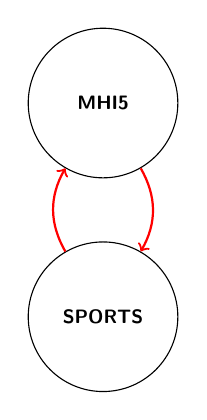
\begin{tikzpicture}[
            node distance=0.8cm,
            main node/.style={circle,draw,font=\scriptsize\sffamily\bfseries,minimum size=1.9cm},
            every edge/.style={draw,thick,->},
        ]
            \node[main node] (mhi5) {MHI5};
            \node[main node, below=of mhi5] (sports) {SPORTS};

            \path[bend left,color=red] (mhi5) edge (sports);
            \path[bend left,color=red] (sports) edge (mhi5);
        \end{tikzpicture}
        \subcaption{Cross-sectional data}
        \label{fig:methods:reverse_causality:cs}
    \end{subfigure}
    \hfill
    \begin{subfigure}[t]{0.49\textwidth}
        \centering
        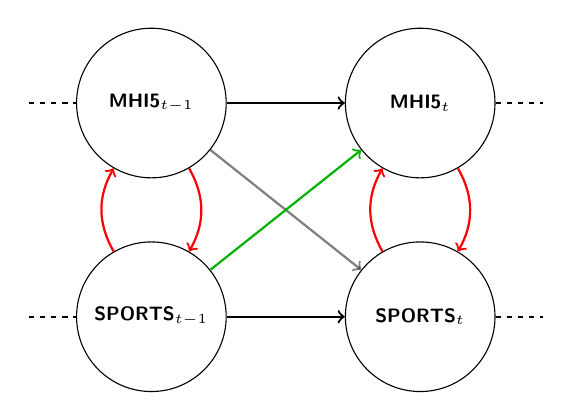
\begin{tikzpicture}[
            node distance=0.8cm,
            main node/.style={circle,draw,font=\scriptsize\sffamily\bfseries,minimum size=1.9cm},
            every edge/.style={draw,thick,->},
            fading line/.style={draw, thick, dotted, dash pattern=on 2pt off 2pt},
        ]
            \node[main node] (mhi5_t) {MHI5$_t$};
            \node[main node, below=of mhi5_t] (sports_t) {SPORTS$_t$};
            \node[main node, left=1.5cm of mhi5_t] (mhi5_t1) {MHI5$_{t-1}$};
            \node[main node, below=of mhi5_t1] (sports_t1) {SPORTS$_{t-1}$};

            \path[bend left,color=red] (mhi5_t) edge (sports_t);
            \path[bend left,color=red] (sports_t) edge (mhi5_t);
            \path[bend left,color=red] (mhi5_t1) edge (sports_t1);
            \path[bend left,color=red] (sports_t1) edge (mhi5_t1);
            \path (mhi5_t1) edge (mhi5_t);
            \path (sports_t1) edge (sports_t);
            \path[opacity=0.5] (mhi5_t1) edge (sports_t);
            \path[color=green!70!black] (sports_t1) edge (mhi5_t);

            \draw[fading line] ([xshift=-0.6cm]mhi5_t1.west) -- (mhi5_t1.west);
            \draw[fading line] ([xshift=-0.6cm]sports_t1.west) -- (sports_t1.west);
            \draw[fading line] (mhi5_t.east) -- ([xshift=0.6cm]mhi5_t.east);
            \draw[fading line] (sports_t.east) -- ([xshift=0.6cm]sports_t.east);
        \end{tikzpicture}
        \subcaption{Panel data. Note the effect of MHI5$_{t-1}$ on SPORTS$_t$ is identified,
        but is considered a nuisance parameter. The green arrow represents the effect of interest}
        \label{fig:methods:reverse_causality:panel}
    \end{subfigure}
    \caption{Graph representations of the hypothesised interactions between MHI5 score and sports.
    Controls are left out for simplicity.
    The green arrow indicates the effect of interest,
    while red arrows indicate unidentified effects}
    \label{fig:methods:reverse_causality}
\end{figure}

While many alternative software pacakges exist, for the present research,
the package \textit{lavaan} in R is used \cite{rosseel2012lavaan}.
This choice was made because \textit{lavaan} is a mature and feature-rich project, whose reliability is exemplified by its
extensive use in the literature.

\section{Structural Equation Modelling}
\label{sec:methods:sem}
SEM can be considered a generalisation of the linear model, where rather than one regression equation which explains
the variability of the regressand with regards to a set of regressors, multiple regression equations are estimated simultaneously
to explain the total covariance structure of all variables involved.
The following will be a minimal introduction into SEM for the purpose of this work,
in which accuracy is sacrificed to some degree in favour of simplicity.
For a full introduction, consider textbooks such as \citeA{kline2023principles}.
While SEM also allows for modelling latent variables in its general form, such constructs are not considered
in this work. This is because the author possesses no a priori knowledge as to what latent constructs might exist, and
\citeA{ludtke2022comparison} find in a simulation study that empirically deciding on latent structures ``is only
of limited usefulness, because the different model[l]ing approaches provide almost equivalent representations of [the data].''

Consider then a vector $z_i$, which contains for individual $i$ the outcome variable of interest $y_i$ as well as
all regressors $x$.
For the purpose of maximum likelihood estimation of the population parameters, note the well-known
likelihood (density) of a single observation
\begin{equation}
    f(z_i; \mu, \Sigma) = (2\pi)^{-\frac{p}{2}} |\Sigma|^{-\frac{1}{2}} e^{-\frac{1}{2}(z_i - \mu)' \Sigma^{-1}(z_i - \mu)},
\end{equation}
where $p$ denotes the dimension of $z_i$ and $\mu$ and $\Sigma$ are respectively the mean and covariance of $z_i$,
and lastly $\pi \approx 3.14$.
Assuming independent observations and dropping the constant, the sample log likelihood is
\begin{equation}
    \label{eq:methods:sample_likelihood}
    l(z) = \sum_{i=1}^N \log(f(z_i; \mu, \Sigma))
    = -\frac{N}{2} \log(|\Sigma|) -\frac{1}{2} \sum_{i=1}^N (z_i - \mu)' \Sigma^{-1} (z_i - \mu),
\end{equation}
which for the purposes of optimisation can be rewritten to an equivalent fit function $F$, defined in terms of
the sample mean $\bar{x}$ and covariance matrix $S$ \cite{preacher2016ml} as
\begin{equation}
    \label{eq:methods:objective_function}
    F(\mu, \Sigma) = \log|\Sigma| + \text{tr}(S \Sigma^{-1}) - \log|S| - p + (\bar{z} - \mu)' \Sigma^{-1} (\bar{x} - \mu),
\end{equation}
with tr($\cdot$) denoting the trace of a matrix and the minimum of $F$ coincides with the maximum likelihood estimate.
Note this fit function does not directly involve any observation $z_i$. Rather it is defined purely in terms of the
sample moments $\bar{z}$ and $S$, which is to say that while \Cref{eq:methods:sample_likelihood} and
\Cref{eq:methods:objective_function} are theoretically equivalent, the latter operates on a higher level of abstraction.

At this stage, the elements of $\mu$ and $\Sigma$ may be estimated directly through numerical optimisation.
Firstly, note that $\mu$ can always be estimated as $\hat{\mu} = \bar{z}$, such that the last term in
\Cref{eq:methods:objective_function} vanishes. It can thus be estimated separately from $\Sigma$,
and because the research question pertains specifically to the variability of variables,
the mean term is ignored in further discussion.
To see how this general multivariate likelihood approach relates to the linear model, consider the very simple example
regression of
\begin{equation}
    \label{eq:methods:simple_regression}
    y = \alpha + \beta_1 x_1 + \beta_2 x_2 + \epsilon.
\end{equation}
From this equation, the model-implied covariances between $y$
and $x_1$ and $x_2$ can be readily defined in terms of the regressor covariances as
\begin{align}
\begin{split}
    \label{eq:methods:covariance_simple_regression}
    \Sigma_{y x_1} &= \beta_1 \Sigma_{x_1} + \beta_2 \Sigma_{x_1 x_2}\text{ and} \\
    \Sigma_{y x_2} &= \beta_1 \Sigma_{x_1 x_2} + \beta_2 \Sigma_{x_2},
\end{split}
\end{align}
where $\Sigma_{x_1}$ ($\Sigma_{x_2}$) denotes the variance of $x_1$ ($x_2$) and $\Sigma_{x_1 x_2}$ denotes the covariance between $x_1$ and $x_2$.
Estimating $\Sigma_{y x_1}$ and $\Sigma_{y x_2}$ thus corresponds directly to estimating $\beta_1$ and $\beta_2$.
In general, the upper-right row of elements of the covariance matrix of $z$ is $\Sigma_{xy} = \Sigma_x \beta$ for
a vector of regressors $x$ and a vector of parameters $\beta$, where $\Sigma_x$ is the covariance matrix of $x$.
For completeness, the diagonal elements of $\Sigma$ are estimated directly as well as the covariance elements between
the regressors, at which point estimating the above regression equation is just a matter of reparametrisation as compared
to estimating the corresponding elements of $\Sigma$ directly; the two approaches are completely equivalent.

A benefit of the higher-level abstraction in SEM as compared the canonical linear model, is that multiple regressions
can be estimated simultaneously. Consider for instance
\begin{align}
\begin{split}
    \label{eq:methods:simultaneous_regression}
    y_1 &= \alpha_1 + \gamma y_2 + \epsilon_1;\\
    y_2 &= \alpha_2 + \beta x + \epsilon_2.
\end{split}
\end{align}
Note the subscripts in $y_1$ and $y_2$ denote different variables altogether,
not necessarily the same variable at different points in time.
Now, the model-implied $\Sigma_{y_1 x} = \gamma \beta \Sigma_x$.
However, because in general the second equation in \Cref{eq:methods:simultaneous_regression} does not fully explain the
variance in $y_2$ ($R^2 < 1$), this may not fully explain the covariance between $y_1$ and $x$.
That is, there may be a residual covariance $\phi_{y_1 x}$, such that $\Sigma_{y_1 x} = \gamma \beta \Sigma_x + \phi_{y_1 x}$.
Note also that with three total variables, there are three covariance elements in $\Sigma$, but $\{\gamma, \beta\}$
constitutes only two parameters to estimate, which is too few parameters to exactly estimate the full covariance structure.
Additionally, $\Sigma_{y_1} = \phi_{y_1} + \gamma \phi_{y_2} + \gamma \beta \Sigma_x$, where
$\phi_{y_1}$ denotes the residual variance of $y_1$ and likewise $\phi_{y_2}$. That is, the variance of $y_1$ is not
just defined in terms of its regressors, but also in terms of its regressors' regressors (and so on).

A general implication of the higher level of abstraction is that while canonically, the linear model has $N - k$ degrees
of freedom if there are $k$ parameters to be estimated, in SEM there are $\frac{p(p+1)}{2} - k$ degrees of freedom
for a model that involves $p$ variables. Note $\frac{p(p+1)}{2}$ is the number of unique elements in the covariance matrix.
For example, the model in \Cref{eq:methods:simple_regression} involves three variables (again, neglecting the mean component),
so again three covariance elements in $\Sigma$. Two of these are implied as in \Cref{eq:methods:covariance_simple_regression},
but because both $x_1$ and $x_2$ only show up as regressors, the model does not imply any structure to their covariance,
and it is simply estimated as $\Sigma_{x_1 x_2} = \phi_{x_1 x_2}$. The residual variance of $y$ is also estimated along
with the two variances of the regressors, which leaves $\frac{p(p + 1)}{2} - k = 6 - 6 = 0$ degrees of freedom. This is
referred to as a model that is just identified.
The model in \Cref{eq:methods:simultaneous_regression} differs in that it implies all three covariances, but with only two
parameters. If the model is not supplemented with $\phi_{y_1 x}$, there is $6 - 5 = 1$ degree of freedom, which is to
say that the model is overidentified.
While the example is trivial, in a more complex model we may exploit overidentification to quantify
whether the proposed model adequately describes the data. In other words, fit indices can be derived from these degrees
of freedom, in some sense analogous to the Sargan-Hansen test for the generalised method of moments.

A model specification in SEM is simply the set of regression pathways and residual variances to be estimated as free
parameters.
SEM lends itself well to the present research, because it necessitates very few restrictions on the model.
This makes it a natural choice for exploring a potentially complex and unknown relationship between variables.
A panel regression fits into the SEM framework by having one regression for each wave of the panel,
i.e. $y_{i,1} = \ldots; y_{i, 2} = \ldots$, and so on. The framework then allows for instance adding autoregressive terms
(dynamic panels), having (co)variances vary across waves or even two-way fixed effects
(i.e. time dummies and individual-specific effects).
Fundamentally, the only restriction imposed by SEM is that the covariance matrix is sufficient to identify the parameters.
Notably, while Arellano-Bond (AB) estimation of dynamic panel models relies on first-differencing the model for identification,
SEM does not and as such it is possible to include time-invariant controls beyond just the catch-all individual-specific effect.
Additionally, AB estimation necessitates a choice of instruments which model validity crucially depends on
\cite{bazzi2013blunt}, and SEM was empirically found by \citeA{leszczensky2022deal} to be more efficient than AB
while also being unbiased in all situations where the model was correctly specified.
Altogether, SEM is the preferred choice for the present study.

\subsection{Fixed and Free Parameters}
\label{sec:methods:fixed_free_parameters}
In \textit{lavaan}, a parameter can either be fixed to a specific value or estimated freely.
There are two forms of parameters, namely regression coefficients and additional (residual) covariances (i.e. $\phi_{x_1 x_2}$).
If a variable is a regressand or if one of its covariances is set as a free parameter, then all of its covariances
must be either estimated through free parameters or fixed to zero to ensure the model-implied covariance matrix is
positive definite.
In that sense, it is meaningful to talk about a variable as whole to be treated as fixed or not.

Treating variables as fixed makes it impossible to examine the covariances between them,
for instance to test whether $\text{Cov}(x_1, x_2) = 0$.
However, for the present work, the choice to treat all regressors as fixed comes naturally,
because the covariance structure between regressors is not relevant to the research question;
doing so improves model parsimony;
and considering fit indices are defined in terms of the degrees of freedom,
a good model fit in terms of the regressors may obscure a poor model fit for the outcome variable,
decreasing the indices' value to the present study.

\subsection{Panel Model Formulation}
\label{sec:methods:model_formulation}
The following model formulation is adapted from \citeA{allison2017maximum}.
In a simplified form, the central regression equation is
\begin{equation}
    \label{eq:methods:model_formulation}
    y_{it} = \alpha_t + \alpha_i + \rho y_{i,t-1} + \beta x_{it} + \omega' w_{it} + \delta' z_i + \epsilon_{it}.
\end{equation}
$y_{it}$ is the MHI5 score of individual $i$ at time $t$ while $\alpha_t$ represents a time dummy,
$x_{it}$ the exercise status, $w_{it}$ is a vector of time-varying controls and $z_i$ a vector of time-invariant controls.
This equation is simplified in the sense that it only contains a single autoregressive (AR) term and a single lag of $x$,
i.e. no distributed lags (DL). This is not a necessary restriction, but is done here for simplicity of
the introduction; the restriction is done away with when developping the model for the present study (\Cref{chap:modelling}).
\Cref{eq:methods:model_formulation} has to be complemented with the initial conditions for $y$.
If only one autoregressive lag is included, only $y_{i,1}$ is required,
but for a higher lag order more initial conditions are required. If distributed lags are included, then likewise for $x$.
A practical implication of this is that the higher the autoregressive (distributed) lag order, the fewer waves
are available for analysis. This is especially relevant in the present study, because the missingness of the MHI5 score
in 2014 means twice as many waves are lost as would be the case if the Health study had been conducted that year.
The fact that time-invariant controls $z_i$ may be included is beneficial for controls that vary so little in time that
treating subsequent values as separate variables causes numerical instability (colinearity). For such a variable,
the first observed (non-NA) value of each individual is used as the time-invariant approximation. While this choice
is ambiguous, the very fact that the variable must be modelled as a time-invariant implies that the exact
choice of approximation matters very little.

The main identifying assumption is \cite{moral2019dynamic}
\begin{equation}
    \label{eq:methods:identifying_assumption}
    E(\epsilon_{it} | y_i^{t-1}, x_i^t, \alpha_t, w_{i}^t, z_i) = 0 \,\forall\,\{i,t\},
\end{equation}
where a superscript $t$ denotes all observations of the corresponding variable up to time $t$.
Verbally, the assumption entails that all included regressors are exogenous.
Note the exogeneity of $x$ is also implied by the ignorability condition (\Cref{eq:methods:ignorability_assumption}).
Furthermore, while all regressors are included in the identifying assumption, if a control is endogenous it simply
leads to inconsistent estimation of the corresponding parameter, that has a weaker influence on the estimation
of the parameter of interest ($\beta$) than endogeneity of $x$ itself, and is thus of lesser concern in practice.
Beyond \Cref{eq:methods:identifying_assumption}, in a random effects specification, the time-invariant controls
must also be uncorrelated with the individual-specific effects, in order to differentiate between $\alpha_i$ and $\delta$.

The coefficient $\beta$ in \Cref{eq:methods:model_formulation} cannot be interpreted directly as the effect that $x$ (exercise)
has at time $t$ on $y$ (MHI5 score), due to the autoregressive behaviour. However, it can be interpreted as a change
in the equilibrium value of $y_{it}$.
In a generalised model with autoregressive coefficients $\{\rho_{l_y} | l_y \in [1, L_y]\}$,
and distributed lag coefficients $\{\beta_{l_x} | l_x \in [0, L_x]\}$, The total effect can be interpreted as follows.
If for an individual $x_{it}$ changes from 0 to 1, i.e. they did not
engage in exercise but have started doing so, they equilibrium value of $y_{it}$ changes by
\begin{equation}
    \label{eq:methods:long_run_effect}
    \frac{\sum_{l_x=0}^{L_x} \beta_{l_x}}{1 - \sum_{l_y=1}^{L_y} \rho_{l_y}}.
\end{equation}
Refer to \Cref{chap:app:long_run_effect} for a derivation.

To briefly note, \Cref{eq:methods:model_formulation} assumes a linear influence of all regressors onto $y$. However, all regressors
are included as dummies, i.e. on a binary scale. For such a scale, linearity holds exactly.
The only exceptions are the autoregressive terms, but since even a small number of autoregressive terms can already
model highly nonlinear temporal behaviour, it is likely a reasonable approximation.

\subsection{Controls and Mediators}
\label{sec:methods:controls_mediators}
As discussed extensively already, the selection of controls is crucial to avoid unmeasured confounders. However,
a second important consideration is the action of mediators. Mediators are variables that explain the effect
of $x$ on $y$, in the sense that $x$ causes some mediator $m$ which causes $y$. An example of a mediator in the present
study might be physical health. If physical health is included as a control in the regression, the interpretation of $\beta$
becomes ``the effect of sports on MHI5 score, \textit{given} the physical health status of an individual.'' However,
improvement of physical health may well be a strong mechanism through which sports affects mental health, which
should very much be included in $\beta$ for the purpose of answering the research question. The subtleties of mediation
are not often discussed in the literature \cite{imbens2024causal}, e.g. \citeA{chekroud2018association} simply include physical health as a control.
Such mediation might be measured directly while still effectively controlling for confoundedness due to the mediator as
in the following, simplified example:
\begin{align}
\begin{split}
    \label{eq:methods:mediation_example}
    y_{it} &= \alpha_y + \beta x_{it} + \eta m_{it} + \epsilon_y; \\
    m_{it} &= \alpha_m + \zeta x_{it} + \epsilon_m.
\end{split}
\end{align}
Then, the total effect of $x$ on $y$ is given as $\beta + \zeta \eta$, the sum of the direct and the indirect effects.
Conveniently, these two regressions may be estimated simultaneously in SEM.

Thus, when determining the controls used, attention must be paid to which variables may be mediators and those should be
modelled as in \Cref{eq:methods:mediation_example}. There is a significant price to be paid in terms of model parsimony
though, as a mediator cannot be a fixed variable, potentially adding many additional parameters to the model.
If a mediator is simply excluded from the regression altogether, this model complexity is avoided, while the indirect
effect (e.g. $\zeta \eta$) is absorbed into the main parameter ($\beta$). However, in doing so, the mediator, in so far
as it is not fully explained by $x$, also functions as a potential unmeasured confounder.
Because it is not clear a priori which approach is preferred, the results for both will be given in the present study.
In this way, it can also be directly examined to which degree the mediators are confounders by comparing
the estimated coefficients $\beta$ between the two approaches.

When multiple mediators are simultaneously modelled, there can be either parallel mediation or serial mediation \cite{hayes2017introduction}.
In parallel mediation (\Cref{fig:methods:mediation_forms:parallel}), the mediators do not influence each other,
whereas in serial mediation (\Cref{fig:methods:mediation_forms:serial}) one mediator causes the next mediator.
If multiple mediators affect each other and the outcome variable as in \Cref{fig:methods:mediation_forms:simultaneous},
there is another form of simultaneity in the model. While this could be modelled with panel data just as the main
simultaneity is modelled in the present study, that would entail significant model complexity.
Instead, the present study models multiple mediators as parallel mediation, which effectively makes the assumption that,
conditional on the set of controls and sports, there is no causal dependence between the mediators.
The residual covariance of the mediators can be estimated in the SEM model to quantify to what extent this approximation
is violated.
Clearly, different dummy levels of the same categorical mediator must be causally dependent, which necessarily
poses a limitation of this study.

\begin{figure}[htbp]
    \begin{subfigure}[t]{0.32\textwidth}
        \centering
        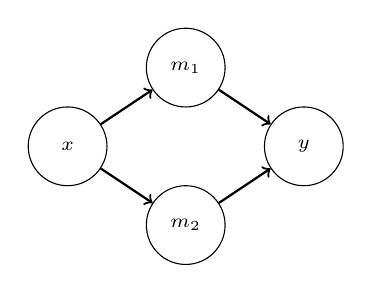
\begin{tikzpicture}[
            node distance=0.4cm,
            main node/.style={circle,draw,font=\scriptsize\sffamily\bfseries,minimum size=1cm},
            every edge/.style={draw,thick,->},
        ]
            \node[main node] (m1) at (0, 2) {$m_1$};
            \node[main node] (m2) at (0, 0) {$m_2$};
            \node[main node] (x) at (-1.5, 1) {$x$};
            \node[main node] (y) at (1.5, 1) {$y$};

            \path (x) edge (m1);
            \path (x) edge (m2);
            \path (m1) edge (y);
            \path (m2) edge (y);
        \end{tikzpicture}
        \subcaption{}
        \label{fig:methods:mediation_forms:parallel}
    \end{subfigure}
    \hfill
    \begin{subfigure}[t]{0.32\textwidth}
        \centering
        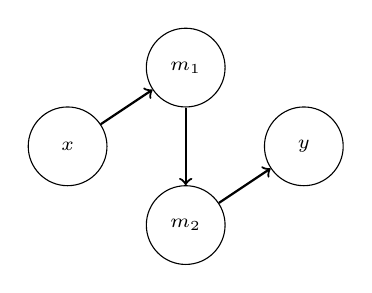
\begin{tikzpicture}[
            node distance=0.4cm,
            main node/.style={circle,draw,font=\scriptsize\sffamily\bfseries,minimum size=1cm},
            every edge/.style={draw,thick,->},
            fading line/.style={draw, thick, dotted, dash pattern=on 2pt off 2pt},
        ]
            \node[main node] (m1) at (0, 2) {$m_1$};
            \node[main node] (m2) at (0, 0) {$m_2$};
            \node[main node] (x) at (-1.5, 1) {$x$};
            \node[main node] (y) at (1.5, 1) {$y$};

            \path (x) edge (m1);
            \path (m2) edge (y);
            \path (m1) edge (m2);
        \end{tikzpicture}
        \subcaption{}
        \label{fig:methods:mediation_forms:serial}
    \end{subfigure}
    \hfill
    \begin{subfigure}[t]{0.32\textwidth}
        \centering
        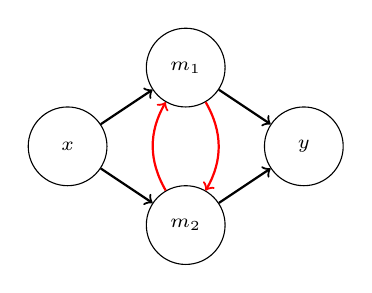
\begin{tikzpicture}[
            node distance=0.4cm,
            main node/.style={circle,draw,font=\scriptsize\sffamily\bfseries,minimum size=1cm},
            every edge/.style={draw,thick,->},
            fading line/.style={draw, thick, dotted, dash pattern=on 2pt off 2pt},
        ]
            \node[main node] (m1) at (0, 2) {$m_1$};
            \node[main node] (m2) at (0, 0) {$m_2$};
            \node[main node] (x) at (-1.5, 1) {$x$};
            \node[main node] (y) at (1.5, 1) {$y$};

            \path (x) edge (m1);
            \path (x) edge (m2);
            \path (m1) edge (y);
            \path (m2) edge (y);
            \path[bend left,color=red] (m1) edge (m2);
            \path[bend left,color=red] (m2) edge (m1);
        \end{tikzpicture}
        \subcaption{}
        \label{fig:methods:mediation_forms:simultaneous}
    \end{subfigure}
    \caption{Graph representations of respectively parallel mediation (a), serial mediation (b), and simultaneity in mediation (c)}
    \label{fig:methods:mediation_forms}
\end{figure}

The simplified example in \Cref{eq:methods:mediation_example} does not include controls or autoregression. In order for the parameters $\zeta$ and $\eta$
to be meaningfully combined, the same set of controls should be present in the mediation regression as in the main
regression. Because of this, all the regressors in the main regression are added to the mediation regression, including
the lagged $y_{i,t-l}$. However, because of the modelling choice of parallel mediation, mediators are not included
in the mediation regressions of other mediators.

An additional concern in mediation is that the mediator may also be a vehicle for the reverse effect.
Just as $\beta$ in \Cref{eq:methods:mediation_example} cannot differentiate between the forward- and reverse effects,
neither can $\eta$ nor $\zeta$. That is, in mediation, there is a concern for both the reverse effect of $y_{it}$ onto
$m_{it}$ and the reverse effect of $m_{it}$ onto $x_{it}$. Just as in \Cref{fig:methods:reverse_causality:panel},
we may measure only lagged effects in both equations, at the cost of model parsimony and only being able to judge the
effect of $x_{i,t-2}$ on $y_{it}$.
If on mechanistic grounds the reverse causality in either equation is expected to be negligible, it can be justified
to measure the instantaneous effect in that regression.
For the interpretation of the long-run effect of $x$, \Cref{eq:methods:long_run_effect} shows that each lag $\beta_l$
has the same influence on the outcome. As such, regardless of the lag structure decided on in mediation, the sum of the
direct and indirect effects can be meaningfully interpreted as the total effect.

Because mediators cannot be treated as fixed variables, a consideration is which of their residual covariances
to set as free parameters.
While there may be autoregressive behaviour for the mediator variables, this is controlled for by
setting the covariance between any two consecutive values of mediators as a free parameter, with these parameters
being allowed to vary freely across time to eliminate all associated degrees of freedom.
An implication of this is that if in reality there is AR behaviour to the mediators, the total
effect of sports through them is underestimated (assuming positive AR coefficients).
The approximation thus maintains type I significance.
The AR nature could also be explicitly modelled, but doing so would make modelling much more complex and error-prone,
so the fact that $\alpha$-significance is maintained justifies accepting the reduced statistical power as a compromise.
Additionally, if a mediator is a categorical variable, there must be a negative correlation between its different
dummy variables, so correlations between different dummy levels of the same variable are also set as free parameters.

\subsection{Fit Indices}
\label{sec:methods:fit_indices}
There is an extensive set of fit indices for SEM models available in the literature. These derive from the degrees of freedom
in various ways. No single fit index is definitive for model fit, so it is prudent to consider multiple indices together
for a more complete view. A canonical set of fit indices is described hereafter. However, first two general remarks are in order.
For one, if a model is just identified, each of these fit indices will always indicate a perfect fit, which is to
say there is then no value in interpreting the indices.
Secondly, these tests do not necessarily provide a way to compare competing models. Considering they all measure the
extent to which the model-implied covariance matrix differs from the sample covariance matrix, if two competing models
involve a different set of variables, the indices cannot be directly compared. That is, if model A fits the sample
covariance matrix $S_A$ better than model B fits $S_B$, it does not necessarily follow that model A is better than model B.
For example, a model which has no controls would likely yield better fit indices because it is a much simpler model
with fewer parameters to be estimated,
but that does not make it the preferred model over a model which includes a set of relevant control variables.
\Cref{sec:methods:cv} will discuss the alternative approach used in this work for model selection.

\subsubsection{$\chi^2$ test}
The $\chi^2$ test is the most general (and the original) fit index used \cite{smith2001primer}. It is a badness-of-fit
test, in the sense that the null hypothesis is that the model explains the data perfectly. To be precise,
the test statistic is the discrepancy between the model-implied covariance matrix and the real covariance matrix,
and a significant test result thus implies a significant discrepancy.
In practice with ML estimation, the test statistic is calculated as
\begin{equation}
    \label{eq:methods:chi2_test_stat}
    \chi^2 = (N - 1) F(\hat{\Sigma}),
\end{equation}
where $F(\cdot)$ is the objective function as in \Cref{eq:methods:objective_function}.
Under the null hypothesis, the statistic is distributed as $\chi^2_{df}$ if the model has $df = \frac{p(p + 1)}{2} - k$ degrees of freedom
\cite{zheng2025enhancing}.

However, a shortcoming of the $\chi^2$ test is that it is sensitive to sample size, in the sense that as
the number of observations $N$ increases, the null is less likely to be maintained. This is not a
desirable property of a fit index, which has given rise to other fit indices \cite{smith2001primer}.
As an alternative, \citeA{joreskog1993lisrel} propose using the ratio $\chi^2 / df$ as an indicator of goodness-of-fit,
where a ratio below 2 represents ``good'' fit and below 3 ``acceptable''. However, this does not fundamentally eliminate
the sensitivity to sample size; rather, it just proposes more lenient critical values.

\subsubsection{Comparative Fit Index}
The Comparative Fit Index (CFI) derives from the $\chi^2$ test. It compares the $\chi^2$ test statistic of the model to that of a baseline model.
While what constitutes the baseline model is subjective (f.i. \citeA{van2021understanding}), typically the baseline model is a
model in which the variances of all variables are estimated, whereas the covariances are not (i.e. fixed to 0).
The statistic is then
\begin{equation}
    \text{CFI} = 1 - \frac{\max(\chi^2 - df, 0)}{\max(\chi^2 - df, \chi^2_b - df_b, 0)}.
\end{equation}
Here, $\chi^2$ and $df$ denote the test statistic and degrees of freedom of the model and the same variables with a
subscript $b$ are those of the baseline model \cite{schermelleh2003evaluating}.
While no analytical distribution is available for this statistic, its value is in the range $[0, 1]$, with a
higher value indicating better fit. It reaches a value of 1 if the ratio of $\chi^2$ to $df$ is less than 1,
and a value of 0 if the baseline model fits the data better than the proposed model.
Typically a cutoff value of $0.95$ is taken to indicate good model fit \cite{hu1999cutoff}.

\subsubsection{Tucker-Lewis Index}
Similar to the CFI, \citeA{schermelleh2003evaluating} define the Tucker-Lewis Index (TLI) as
\begin{equation}
    \text{TLI} = \frac{\chi_b^2 / df_b - \chi^2 / df}{\chi_b^2 / df_b - 1}.
\end{equation}
While not strictly confined to the range of $[0, 1]$, the TLI is typically in that range, only exceeding it
if the baseline model outperforms the proposed model, or if model fit is so good as to make $\chi^2 < df$.
Again, a higher TLI is better, and the cutoff for good fit is taken from \citeA{hu1999cutoff} as 0.95.

\subsubsection{Root Mean Square Error of Approximation}
The Root Mean Square Error of Approximation (RMSEA) measures the discrepancy between the model-implied- and
sample covariance matrices per degree of freedom,
roughly defined as the root mean square difference between the two \cite{schermelleh2003evaluating}.
It improves on the $\chi^2$ statistic by compensating for the degrees of freedom and the sample size.
\begin{equation}
    \text{RMSEA}^2 = \frac{\max(\chi^2 - df, 0)}{df(N - 1)}.
\end{equation}
The RMSEA has a lower bound of 0 and no upper bound, with a lower RMSEA representing better fit.
We use a cutoff of 0.06 to indicate good fit \cite{hu1999cutoff}.

\subsubsection{Standardised Root Mean Square Residual}
Lastly, the Standardised Root Mean Square Residual (SRMR) is defined most explicitly in terms of $S - \hat{\Sigma}$
without considering degrees of freedom, namely as \cite{schermelleh2003evaluating}
\begin{equation}
    \text{SRMR}^2 = \frac{\sum_{i=1}^p\sum_{j=1}^i (\frac{S_{ij} - \hat{\Sigma}_{ij}}{S_i S_j})^2}{p(p+1)/2}.
\end{equation}
The term being summed is the (square) discrepancy between $S$ and $\hat{\Sigma}$, standardised with respect to the sample standard
deviations $S_i$ and $S_j$ to eliminate dependence on the scale of variables.
Again, it has no upper bound but is bounded below by 0, and lower values indicate better fit.
The cutoff used is 0.08 \cite{hu1999cutoff}.

\subsection{Cross Validation}
\label{sec:methods:cv}
For the sake of model selection, a model-agnostic measure of model fit is required. To this end, we may borrow from the
machine learning literature and use out-of-sample forecasting accuracy through cross validation.
This approach can be used to compare any two models, including non-nested ones, and is a fit measure more akin to those
used in canonical linear modelling.
However, as mentioned before, when comparing different autoregressive lag orders, the lower lag order will have
more waves available. It is likely that a model fit to a larger number of waves has a worse fit due to slight
unmodelled heterogeneity across the waves, making the comparison between models unfair. Because of this, only the last
available wave (2023) is used for cross validation, both for fitting the models as well as for determining the forecasting
accuracy. It does not necessarily hold that the model that best fits the final wave is the one that best fits
the data as whole, but it is nevertheless taken as a necessary and reasonable approximation.

In model selection, accuracy must be balanced with parsimony. To this end, the decision rule used is the 1-$\sigma$ rule,
where the model chosen is the simplest model whose out-of-sample forecasting accuracy is within one standard deviation
of the best-performing model. Specifically, across the $v$ folds, the root mean square prediction error (RMSPE)
$\mu_{\text{RMSPE}}$ is calculated, along with the standard deviation of this prediction error across the folds,
$\sigma_{\text{RMSPE}}$. The simplest model whose $\mu_{\text{RMSPE}}$ is below the optimal model's
$\mu_{\text{RMSPE},opt} + \sigma_{\text{RMSPE},opt}$ is selected.
In this, the number of folds $v$ plays a critical role, as when more folds are used, the training sets are larger
and the testing sets are smaller, which generally leads to lower $\mu_{\text{RMSPE}}$. Typical values are $v = 5$ or
$v = 10$. The dataset at hand is large, but considering the high percentage of missing data, a smaller number for
$v$ is preferred to avoid unrepresentative test sets, so $v = 5$ is used.
To improve the accuracy of the estimated $\mu_{\text{RMSPE}}$ and $\sigma_{\text{RMSPE}}$, this cross validation
is repeated $R$ times with different random folds in each repetition and the average estimates is taken.
Here, the larger $R$ the better, but $R = 50$ is chosen to balance precision and computational tractability.
Because uncertainty in the estimates has a significant impact on the 1-$\sigma$ decision rule,
the uncertainties in the estimates of $\mu_{\text{RMSPE}}$ and $\sigma_{\text{RMSPE}}$ are calculated as the standard
deviation of the respective estimates across the repetitions divided by the square root of $R$.
The uncertainty of the decision rule threshold is then found by quadratically adding these two uncertainties.
There is the possibility that the model used is not identified or numerically unstable for a given split due to the high
degree of missingness. When this occurs, the results for the current repetition are discarded and another repetition is
done.

\subsection{Full Information Maximum Likelihood}
\label{sec:methods:fiml}
SEM, at least when combined with maximum likelihood estimation, provides a natural way to handle (MAR) missing data in the
form of Full Information Maximum Likelihood (FIML) \cite{arbuckle2013full}.
The basic premise of FIML is that if a variable is missing for some observation, that observation provides no information
as to how the missing variable relates to other variables, but it still provides information for the remaining variables.
Formally, consider estimation of the covariance matrix $\Sigma$ of the vector $x' = (x_1, x_2, x_3)$.
Because the total sample likelihood (\Cref{eq:methods:sample_likelihood}) is the product of the likelihood of each observation,
we need not necessarily use the same likelihood specification for each observation.
If for some observations $x_3$ is missing, their contribution to the likelihood is simply calculated with the two-dimensional
covariance matrix of the sub-vector $(x_1, x_2)'$.
In this way, FIML uses all information available in the dataset, hence its name. It can be applied to regressors
as well as to regressands, making it highly valuable for the present study.
It is not, however, a solution to a variable completely missing from the data, as is for instance the case with the
missing Health study in 2014. In that case there is no information in the sample altogether, i.e. the sample covariance
is not known and thus cannot be fit to.

\textit{Lavaan} provides the option to apply FIML only to the endogenous variables or to all variables.
If FIML is only applied to the endogenous variables, listwise deletion is applied for those cases where the exogenous
variables are missing. As doing so would eliminate a large portion of the data, FIML is used for all variables in the dataset.

\subsection{Normality and Robust Maximum Likelihood}
\label{sec:methods:normality_mlr}
The derivation of the objective function in \Cref{eq:methods:objective_function} heavily relies on the assumption
of normality. However, while this assumption might hold approximately for the MHI5 score, it clearly does not hold
for all binary regressors. This is of no concern for exogenous variables, as their covariances are simply fixed
to the sample covariance, but it does implicate the parameter of interest, namely the effect of exercise on MHI5.
Even so, \citeA{knief2021violating} find that the normal estimator still behaves well in terms of bias and
efficiency. They even argue that it may be preferable to violate the assumption of normality over using specific
techniques to adjust for non-normality, as those are error prone.
Nevertheless, it would seem worthwhile to use a robust approach to maximum likelihood estimation that are readily
available in \textit{lavaan}. While multiple choices exist, ML with Huber-White standard errors is used in
this study (often referred to as ``MLR''),
as it was found to perform well in the face of nonnormality \cite{zhong2011bias},
while still allowing for the use of FIML which some robust alternatives prohibit.
With MLR in \textit{lavaan}, a robust alternative to the $\chi^2$ statistic is also calculated as in \citeA{satorra2001scaled},
which means the $\chi^2$ statistic but also all the fit indices that derive from it are robust.
In practice it was found that bootstrap standard errors align well with the standard errors implied by MLR estimation,
whereas standard errors with regular maximum likelihood were appreciably smaller, which corroborates the decision to prefer
robust estimation.


\chapter{Model Development}
\label{chap:modelling}
\section{Regressors}
\label{sec:modelling:regressors}
As covariates, we include a basic set of sociodemographic variables available in the Background Variables of the LISS panel,
namely age, ethnicity, gender, marital status, education level, employment status and net household income.
While the first three are (largely) determined at birth, the last four might be hypothesised as mediators based on the literature
(\citeA{spiker2014mental,hjorth2016mental,frijters2014effect,thomson2022income} respectively).
However, all of these variables were found to vary so little in time that including them as time-variant covariates caused
numerical instability, so they could only be included as time-invariants. This precludes modelling them as mediators
of the time-variant variable sports,
but the fact that they vary so little indicates that their effect as mediators could only be weak ($\zeta$ must be small),
so the error in estimating the total effect due to not modelling them as mediators could only be marginal.
Beyond this set, based on the literature and availability in the data, we include (self-reported) physical health
and presence of diagnosed diseases as additional mediators \cite{westcott2012resistance}.
While the Health study also queries more nuanced variables like hospital admittance and medication use, these are
highly correlated with general health and disease status (e.g. $\rho \approx 0.55$ for medication use and disease status),
and are thus excluded for the sake of parsimony, noting the significant increase in complexity that mediators bring.
Both of these mediators are binary variables (after dummy encoding), so a logit regression is preferred.
However, while \textit{lavaan} does support binary variables, it is not possible to use the MLR estimator nor FIML,
and crucially, numerical stability was poor when treating the mediators as binary variables.
Thus, the approximation is made that they are linear variables (i.e. variables on a ratio scale).
By virtue of the Taylor approximation, this approximation holds reasonably if the estimated effect sizes of the regressors
are moderate.

Body composition, aerobic fitness and disease have been found to affect exercise adherence \cite{abernethy2012biophysical}.
For both mediators thus, the reverse effect of the mediator on sports engagement is of concern.
Additionally, the reduced self-efficacy associated with poor mental health is associated
with bad habits like eating disorders \cite{oellingrath2014eating}, influencing physical health.
The same mechanism of also pertains to mediation through disease status, as diet is known to be a
significant determinant of immune function \cite{childs2019diet}.
The conclusion is therefore that for both mediators, reverse causality is of concern for both steps of the mediation
action, necessitating that only the lagged influence of regressors on regressands is considered.

Because only the long-term effect of sports on mental health is considered (recall \cref{sec:methods:reverse_causality}),
it would be natural to use the cumulative years that someone has exercised as the variable of interest, rather than the
yearly exercise status. However, because it is not known how many years one has exercised at the time of joining this panel,
this variable can only be roughly approximated through a running sum. Additionally, information missing in one year would
complicate using the variable in all future years.
As such, sports is used directly, while examining different orders of the distributed lags to model effects beyond
one year ahead.

This study chooses to not include individual-specific effects $\alpha_i$ in the model. This is because while they help justify
the ignorability assumption through eliminating unmeasured confounders, they also potentially obscure the effects of time-invariant mediators,
which equally invalidate the findings. The approach is thus instead to model individual-specific variability through the
time-invariant controls $z_i$. Additionally, inclusion of fixed effects entails estimating $N$ additional parameters
(the incidental parameter problem). Since it is likely that $N > \frac{p(p + 1)}{2}$, the model would not be identified.
That being said, nothing prevents modelling random effects. In fact, this is commonly done in
SEM, see for instance \citeA{heck2001multilevel}. However, the author leaves it as an avenue for further research.

As a minor final comment, some dummy levels of controls were excluded, because they occurred so infrequently in the data
that including them as regressors led to numerical instability.
These were a gender of ``other'' and, perhaps surprisingly, a household income between 15\,000 and 50\,000.

\section{Lag Selection}
\label{sec:modelling:lags}
For determining the autoregressive lag order $L_y$ and the distributed lag order $L_x$, cross validation was run as
described in \cref{sec:methods:cv}.
However, for computational tractability, mediators were not modelled explicitly as such but simply included as controls.
This should have only a minor impact on forecasting MHI5, but makes a higher number of repeats $R = 50$ feasible.
It is assumed that the optimal model structure found in this way also applies when mediation regressions are also
included.
Additionally, it was found that only applying FIML to the endogenous variables yielded very similar parameter estimates
and thus similar forecasts. To then further improve computational tractability in cross validation, listwise deletion
was used for the exogenous variables (i.e. the controls).

Both $L_y$ and $L_x$ were varied from 1 to the highest number available based on the data.
Due to the missing Health study in 2014, this is $L_y = 8$, and because the sports has only been included since 2012,
$L_x = 11$.
The optimal $L_y$ is first estimated, as it has a more profound role in the model than the distributed lag.
When doing so, $L_x = 1$ is used as the most minimal model. When optimising $L_x$, the optimal set of AR lags is used.
It could technically be possible that a better model fit is found when not including all lags between the lowest
and the highest lag, for instance having the set of lags $\{1, 2, 4\}$. This was however not tested as it seems improbable
given the mechanisms at play, and thus would likely be overfitting.
\Cref{fig:modelling:cv_lags} visualises the found RMSPEs.

\begin{figure}[htbp]
    \centering
    \caption{Cross validated out-of-sample forecasting accuracy for varying lag orders, measured by root mean square error.
    Errorbars are standard deviations of accuracy across folds. The horizontal line represents the 1-$\sigma$ decision rule.
    The smaller errorbars represent uncertainty in $\mu_{\text{RMSPE}} + \sigma_{\text{RMSPE}}$}
    \label{fig:modelling:cv_lags}
    \begin{subfigure}[t]{0.49\textwidth}
        \centering
        \includesvg[width=\textwidth]{figures/modelling/cv_AR.svg}
        \vspace{0.1em}
        \subcaption{$\mu_{\text{RMSPE}}$ for varying maximum autoregressive lag $L_y$}
    \end{subfigure}
    \hfill
    \begin{subfigure}[t]{0.49\textwidth}
        \centering
        \includesvg[width=\textwidth]{figures/modelling/cv_DL.svg}
        \vspace{0.1em}
        \subcaption{$\mu_{\text{RMSPE}}$ for varying maximum distributed lag $L_x$}
    \end{subfigure}
\end{figure}

For the autoregressive lags, the most complex model with AR lag order $L_y = 8$ performs best. The decision rule
then indicates $L_y = 3$ is best, though the estimation uncertainty makes $L_y = 4$ also worth considering.
Recalling that the cross validation findings may not generalise as it is only done on the data for 2023, and noting that
simpler models generalise better, $L_y = 3$ is chosen.
For the distributed lags, while the prediction error trends downwards with increasing model complexity,
the model with $L_x = 1$ is clearly favoured.

It should be noted that both figures show that especially with more complex models, $\sigma_{\text{RMSPE}}$ and the estimation uncertainties
are significantly larger. This is likely evidence for some of the testing folds having erratic values.
While this can potentially be fixed by stratifying testing folds on missingness, experimenting with fold counts other than 5 or
through increasing the number of repetitions $R$, the the impact of these outliers on the decision rule is minor and does
not influence the outcome, so this was not done.

\section{Fixing Parameters across Time}
\label{sec:modelling:parameter_fixing}
In the SEM model formulation, a fixing a parameter across time is effected by imposing an equality constraint on the
parameters to be estimated.
It is possible to quantify the validity of these parameter constraints in terms of the $\chi^2$ statistic.
Namely, when relaxing such a constraint, a single degree of freedom is won. The improvement (decrease) in the $\chi^2$
statistic can then be compared to a $\chi^2(1)$ distribution for statistical significance, where the null is
that the parameter constraint is appropriate.
When performing this test on the 180 constraints imposed in the model without mediators, the highest found test
statistic was for the first autoregressive parameter in wave 2023. It was $11.6$, which is greater than the critical
value of $3.84$. However, multiple testing ought to be considered.
When simply applying a Bonferroni correction for doing 180 tests, the critical value becomes $13.2$, thus none of the
imposed constraints are put into question.
While an alternative correction would maintain more power and might reject the null, especially because
the Bonferroni correction assumes the tests are independent but because the parameters are fixed across multiple
regressions this is clearly not true, it should also be noted that
the $\chi^2$ test's sensitivity to sample size means the null is rarely maintained. As such, the conclusion is drawn
that fixing the (regression) parameters across time is appropriate.
It is assumed that this finding generalises to the model with mediators.

However, the same cannot be said for the residual variances of $y$. Because of the way that SEM estimates the
parameters when regressands are also used as regressors (as in \cref{eq:methods:simultaneous_regression}),
the residual variance of MHI5 in 2023 is smaller than that the earlier waves. The model could be adjusted
to prevent this by setting the residual variances between MHI5-values that don't occur in the same regression as free
parameters (eliminating associated degrees of freedom). However, the residual variances are not of interest for the present
research question, so for simplicity's sake the residual variances of MHI5 are simply not constrained across time.


\chapter{Results and Discussion}
\label{chap:results_discussion}
For the definitive models in \textit{lavaan} syntax, refer to the programming code (\cref{chap:app:code}).

\section{Excluding Mediation}
\label{sec:results:no_mediation}

To reiterate, in this approach mediation regressions are not included and neither are the mediators included as regressors,
gaining model parsimony at risk of violating the ignorability assumption.
The regression parameters are listed in \cref{tab:results:basic_regression}. Since besides the autoregressive
terms each variable included is a binary variable, the parameters can be interpreted as the percentage point change
in mental wellbeing (MHI5) as a result of that variable.
In general, very few estimated parameters are significant, and even those that are represent only a marginal impact,
no greater than $1.4$ points for an income above € 50\,000 as compared to no income. Contrast this with the interquartile
range in MHI5 of about $20$ (\cref{fig:data:sample_moments_y_x}).

The results may especially be put into question for the very small instantaneous association between sports and MHI5.
While statistically significant, an average improvement of $0.48$ on a scale of 0 to 100 for individuals who exercise
is in stark contrast with cross-sectional analyses in the literature. Recall for instance the 43\% decrease in days of poor mental
health found in \citeA{chekroud2018association}, or the review by \citeA{noetel2024effect} who find effect sizes of between
$0.2$ and $0.8$ times the sample standard deviation on various measures.
The estimated long-term effect of exercise is highly insignificant ($p = 0.888$), and hence the null hypothesis that
no such long-term benefit exists is maintained.

The CFI and TLI are just above $0.95$, indicating good fit, while the RMSEA and SRMR are far below their respective
cutoff values, which reflects excellent fit. Altogether, the model fit then appears quite good.
In time series analysis, it is also customary to examine the stability of the data, as stability is typically a necessary
assumption for estimation. While SEM does not rely explicitly on this assumption, absence of stability would at least make the
assumption that parameters are constant in time contentious, and the derivation of the long-term effect as a change
in equilibrium value (\cref{eq:methods:long_run_effect}) does rely on stability.
Based on the reported autoregressive coefficients, the roots of the characteristic polynomial are $z_1 = 1.10$,
$z_2 = -1.16 + 1.78i$ and $z_3 = -1.16 - 1.78i$, which all fall decidedly outside of the unit circle,
indeed indicating a stable time series.

\newcolumntype{L}{>{\hspace*{3mm}}l}
\begin{table}[htbp]
    \centering
    \caption{Parameter estimates and fit indices for the base regression.
    Estimates are changes in mean MHI5-scores with respect to the dummy level in parentheses.
    Fit indices are robust variants where applicable}
    \label{tab:results:basic_regression}
    \begin{tabular}{
        L
        S[table-format=2.3] % three decimals, two digits before
        S[table-format=2.3]
        S[table-format=2.3]
        S[table-format=1.3]
    }
    \toprule

    \textbf{Regressor} & \textbf{Estimate} & \textbf{Std. Error} & \textbf{z-value} & \textbf{p-value} \\

    \midrule

    MHI5$_{t-1}$                    & 0.397     & 0.007 & 54.254    & 0.000 *** \\
    MHI5$_{t-2}$                    & 0.248     & 0.008 & 30.737    & 0.000 *** \\
    MHI5$_{t-3}$                    & 0.202     & 0.007 & 26.939    & 0.000 *** \\

    sports$_t$                      & 0.432     & 0.177 & 2.746     & 0.013 * \\
    sports$_{t-1}$                  & -0.025    & 0.177 & -0.140    & 0.888 \\

    \multicolumn{5}{l}{\textit{age} (below 18 years)} \\
    18-24 years                     & -0.343    & 0.372 & -0.923    & 0.356 \\
    25-39 years                     & -0.107    & 0.438 & -0.244    & 0.807 \\
    40-66 years                     & 0.700     & 0.443 & 1.579     & 0.114 \\
    over 67 years                   & 0.331     & 0.490 & 0.676     & 0.499 \\

    \multicolumn{5}{l}{\textit{income} (none)} \\
    below € 15\,000                 & 1.042     & 0.536 & 1.944     & 0.052 $^+$ \\
    over € 50\,000                  & 1.331     & 1.178 & 1.129     & 0.259 \\

    \multicolumn{5}{l}{\textit{immigration status} (Dutch)} \\
    first generation western        & -0.688    & 0.257 & -2.683    & 0.007 ** \\
    first generation non-western    & -0.959    & 0.268 & -3.576    & 0.000 *** \\
    second generation western       & -0.403    & 0.223 & -1.809    & 0.070 $^+$ \\
    second generation non-western   & -0.245    & 0.277 & -0.885    & 0.376 \\

    \multicolumn{5}{l}{\textit{gender} (female)} \\
    male                            & 0.562     & 0.103 & 5.474     & 0.000 *** \\

    \multicolumn{5}{l}{\textit{marital status} (divorced)} \\
    married                         & 0.155     & 0.178 & 0.873     & 0.383 \\
    never been married              & -0.651    & 0.207 & -3.139    & 0.002 ** \\
    separated                       & -0.813    & 0.859 & -0.947    & 0.344 \\
    widow or widower                & 0.337     & 0.289 & 1.167     & 0.243 \\

    \multicolumn{5}{l}{\textit{education level} (havo-vwo)} \\
    hbo                             & -0.176    & 0.193 & -0.914    & 0.361 \\
    mbo                             & 0.021     & 0.196 & 0.110     & 0.913 \\
    primary school                  & -0.382    & 0.273 & -1.401    & 0.161 \\
    vmbo                            & -0.056    & 0.205 & -0.273    & 0.785 \\
    university (wo)                 & -0.436    & 0.218 & -0.273    & 0.046 * \\

    \multicolumn{5}{l}{\textit{employment status} (employed)} \\
    homemaker                       & -0.510    & 0.195 & -2.618    & 0.009 ** \\
    retired                         & 0.063     & 0.191 & 0.327     & 0.744 \\
    student                         & -0.594    & 0.337 & -1.764    & 0.078 $^+$ \\
    unable to work                  & -1.409    & 0.313 & -4.505    & 0.000 *** \\
    unemployed                      & -0.415    & 0.365 & -1.137    & 0.256 \\

    \midrule

    Observations    & \multicolumn{4}{l}{12920} \\
    Parameters      & \multicolumn{4}{l}{225 (180 equality constraints)} \\
    $\chi^2$        & \multicolumn{4}{l}{1530.6 ($df = 270$, $p = 0.000$)} \\
    CFI             & \multicolumn{4}{l}{0.956 (cutoff = 0.95)} \\
    TLI             & \multicolumn{4}{l}{0.951 (cutoff = 0.95)} \\
    RMSEA           & \multicolumn{4}{l}{0.019 (cutoff = 0.06)} \\
    SRMR            & \multicolumn{4}{l}{0.026 (cutoff = 0.08)} \\

    \bottomrule

    \multicolumn{5}{l}{\textit{Significance levels:} $^+$ 0.10, * 0.05, ** 0.01, *** 0.001} \\
\end{tabular}
\end{table}

\section{Including Mediation}
\label{sec:results:mediation}

The main findings of interest in the mediation analysis are to what extent the effect is explained by the mediators,
and the degree to which the mediators confounded the result as indicated by the change in the estimated total effect.
The model contains an overwhelming number of parameters, which would be difficult to interpret.
Hence, \cref{tab:results:mediation_regression} lists the main parameters of interest, namely those of sports
in the mediation regressions and those of sports and the mediators in the main regression.
For the complete parameter estimates, refer to \cref{chap:app:mediation_regression}.
\Cref{tab:results:mediation_total_effect} reports the total effects derived from the results.

The instantaneous effect of sports as well as the (direct) lagged effect are now notably more negative than when no mediators
are included, changing by $-0.390 \pm 0.24$ and $-0.142 \pm 0.25$ respectively. This points towards there indeed being a
positive effect through the mediators, with the large estimated effects of physical health showing it especially is an important
factor. The change in the instantaneous association also provides some evidence for mediation of the reverse
action, i.e. that being sick or being in poor physical health decreases chance to exercise, although the difference
is not significant ($p = 0.110$ based on the above numbers).
The effect of lagged sports is insignificant at $-0.167 \pm 0.172$ with a p-value of $0.332$.

Being ill decreases mental wellbeing ($p < 0.001$), but only moderately with a $-1.384$ percentage point change
in MHI5 on average.
Interesting is that being being ill last year has a similarly large but positive effect of $1.474$ percentage points,
indicating that having recovered from a disease improves wellbeing and/or that having just fallen ill is associated
with a larger mental burden than having been ill for a longer time.
We do not find a significant long-term effect of exercise on disease status ($p = 0.155$).
This indicates that exercise does not seem to strengthen the immune system in the long run,
and because the LISS panel also queries bone fractures, exercise may also not have a beneficial effect towards
strengthening the skeleton, regardless of for instance \citeA{hong2018effects}'s findings that exercise
increases bone mass.
However, because this includes various forms of disease simultaneously, the finding does not preclude a positive effect of exercise on
some forms of disease as in \citeA{westcott2012resistance}, if those effects are offset with a negative effect on other forms
of disease.
In total, the causal long-term effect of physical exercise on mental wellbeing as moderated by disease is $-0.009$
percentage points, which is statistically insignificant at $p = 0.168$.

Physical health is found to have by far the greatest impact on MHI5 of any regressor,
with effect sizes as high as $-19.840$ percentage points.
There is a clear trend that worse physical health is associated with worse mental health.
Strikingly however, the lagged effects all have an opposite sign, that is, a positive association with mental wellbeing.
This is evidence of a similar rebound mechanism as with disease, where having recently had physical health improve is
cause for happiness, and vice versa.
Exercise generally relates to better physical health, but effect sizes are modest, with the greatest change found
being that exercise is associated with a 4.0\% increased probability of being in good physical health.
Lagged exercise significantly decreases probability of moderate physical health ($-2.4\%$, $p < 0.001$) while increasing
the probability of very good mental health ($2.3\%$, $p < 0.001$).
Interesting is the finding that the probabilities of reporting poor or excellent health
are only weakly influenced by instantaneous and lagged sports, indicating that at the extremes of physical health,
the effects of sports are overwhelmed by the effects of other (unmeasured) factors.
Combined with the large detrimental effect of last year's physical health on MHI5, we find a causal effect
of $-0.117 \pm 0.022$ percentage points MHI5 ($p < 0.001$). The negative sign of this effect is contrary to expectations based on the
literature, which find a positive effect if any. This oddity is due to the aforementioned rebound effect.

MHI5 is found to be positively predicted instantaneously by being overweight ($1.241$, $p = 0.025$) and
being obese ($1.232$, $p = 0.041$), both as compared to being underweight. These associations are actually more positive
than the effect of being normal weight, though not statistically significantly so.
Because we are controlling for physical health and disease status, these findings suggest that the effects of a negative
body image are more significant in underweight individuals than in overweight or obese individuals.
There is a significant instantaneous association between sports and being normal weight ($1.7\%$, $p = 0.009$)
as well as being obese ($-1.8\%$, $p < 0.001$), with no association found for being underweight or overweight.
Lagged exercise only has a significant effect on the probability of being normal weight, increasing it by $0.9\%$ ($p = 0.038$),
with all other effects trending towards decreased probabilities.
This small change leads to a total effect of sports on MHI5 as mediated by BMI of $0.002$ with an associated p-value of $0.095$.

Combining the direct effect and the effects through the three mediators, we conclude that engaging in exercise decreases
MHI5 on average by $-0.290 \pm 0.174$ percentage points ($p = 0.095$), equivalent to a long-run effect of $-1.45$
percentage points.
The total effect is but weakly significant because the effect through physical health is overshadowed by the uncertainty
in the direct effect.
$-0.290$ is a small impact as compared to the IQR of $20$ percentage points, and considering the weak significance
the negative sign should not be given much interpretation beyond the aforementioned rebound effect in physical health.
The total effect is not very different from the direct effect of $-0.025$ found in in the analysis without mediation
(\cref{tab:results:basic_regression}), from which we may conclude that the mediators did not appear to have a significant
effect as unmeasured confounders.

In terms of the model quality, the fit indices are appreciably worse than in the simpler model, as is to be expected
considering the significantly increased complexity. Note there are 3100 model parameters compared to the 225 before.
While the RMSEA of $0.027$ still indicates good and in fact excellent fit, the SRMR of $0.089$ barely does not and the
CFI and TLI are around $0.85$ which is decidedly smaller than the cutoff value for good fit of $0.95$.
Considering the majority of the non-fixed variables are the mediators, the relatively poor fit is already an indicator
that the assumption of parallel mediation is not accurate,
i.e. that there are a lot of relationships between the mediators that are not accurately modelled.
This is confirmed in the estimated residual covariances between different dummy levels of the same mediator,
which are all statistically significant with $p \ll 0.01$ and z-scores as high as $70$.
That being said, the relationships between mediators are only of interest in so far as they alter estimations
of the parameters of interest (\cref{tab:results:mediation_regression}), which is likely not an overwhelming influence.
Combined with the acceptable to great SRMR and RMSEA, the results are taken to be sufficiently accurate for the
purpose of answering the research question.

Out of the parameters of interest, the largest effect size found in mediation regressions is $0.044$.
Some other parameters are larger, like $0.283$ for the effect of being over 67 years old on disease status,
but none of the parameters of interest are as large and the vast majority of parameters is below $0.050$,
so the approximation of using linear models over a logit analysis is largely justified.
The AR parameters are very similar to those in the model without mediation, so again time series stability is
expected, confirmed by the roots of the characteristic polynomial $z_{1, 2} = -1.19 \pm 1.85i$ and $z_3 = 1.13$
falling outside the unit circle again.

\begin{table}[htbp]
    \scriptsize
    \centering
    \caption{Parameters of interest in the mediation analysis; controls are not reported.
    Regressands are in bold}
    \label{tab:results:mediation_regression}
    \begin{tabular}{
        L
        S[table-format=2.3]
        S[table-format=2.3]
        S[table-format=2.3]
        S[table-format=1.3]
    }
    \toprule

    \textbf{Regressor} & \textbf{Estimate} & \textbf{Std. Error} & \textbf{z-value} & \textbf{p-value} \\

    \midrule

    \multicolumn{5}{l}{\textbf{MHI5$_t$}} \\
    MHI5$_{t-1}$                    & 0.391     & 0.007 & 54.301    & 0.000 *** \\
    MHI5$_{t-2}$                    & 0.227     & 0.008 & 29.093    & 0.000 *** \\
    MHI5$_{t-3}$                    & 0.182     & 0.007 & 25.401    & 0.000 *** \\

    sports$_t$                      & 0.042     & 0.168 & 0.249     & 0.803 \\
    sports$_{t-1}$                  & -0.167    & 0.172 & -0.969    & 0.332 \\

    disease status$_t$              & -1.384    & 0.216 & -6.398    & 0.000 *** \\
    disease status$_{t-1}$          & 1.474     & 0.221 & 6.677     & 0.000 *** \\

    \multicolumn{5}{l}{\textit{physical health}$_t$ (excellent)} \\
    good                            & -6.366    & 0.310 & -20.566   & 0.000 *** \\
    moderate                        & -12.818   & 0.402 & -31.907   & 0.000 *** \\
    poor                            & -19.840   & 0.861 & -23.050   & 0.000 *** \\
    very good                       & -2.785    & 0.283 & -9.859    & 0.000 *** \\
    \multicolumn{5}{l}{\textit{physical health}$_{t-1}$ (excellent)} \\
    good                            & 2.952     & 0.342 & 8.631     & 0.000 *** \\
    moderate                        & 6.176     & 0.422 & 14.642    & 0.000 *** \\
    poor                            & 10.746    & 0.820 & 13.102    & 0.000 *** \\
    very good                       & 1.694     & 0.320 & 5.288     & 0.000 *** \\

    \multicolumn{5}{l}{\textit{BMI}$_t$ (underweight)} \\
    normal weight                   & 0.306     & 0.518 & 0.591     & 0.554 \\
    overweight                      & 1.241     & 0.552 & 2.247     & 0.025 * \\
    obese                           & 1.232     & 0.603 & 2.042     & 0.041 * \\
    \multicolumn{5}{l}{\textit{BMI}$_{t-1}$ (underweight)} \\
    normal weight                   & 0.347     & 0.567 & 0.612     & 0.541 \\
    overweight                      & -0.020    & 0.602 & -0.033    & 0.973 \\
    obese                           & 0.207     & 0.656 & 0.315     & 0.752 \\

    \midrule

    \multicolumn{5}{l}{\textbf{Disease status$_t$}} \\
    sports$_t$                      & -0.007    & 0.004 & -1.608    & 0.108 \\
    sports$_{t-1}$                  & -0.006    & 0.004 & -1.423    & 0.155 \\

    \midrule

    \multicolumn{5}{l}{\textbf{Physical health$_t$} (excellent)} \\
    good                            & \multicolumn{4}{l}{} \\
    \hspace{3mm} sports$_t$         & -0.009    & 0.007 & -1.400    & 0.162 \\
    \hspace{3mm} sports$_{t-1}$     & -0.009    & 0.007 & -1.400    & 0.162 \\

    moderate                        & \multicolumn{4}{l}{} \\
    \hspace{3mm} sports$_t$         & -0.020    & 0.007 & -3.007    & 0.003 ** \\
    \hspace{3mm} sports$_{t-1}$     & -0.024    & 0.005 & -4.906    & 0.000 *** \\

    poor                            & \multicolumn{4}{l}{} \\
    \hspace{3mm} sports$_t$         & -0.007    & 0.002 & -4.610    & 0.000 *** \\
    \hspace{3mm} sports$_{t-1}$     & 0.001     & 0.002 & 0.957     & 0.339 \\

    very good                       & \multicolumn{4}{l}{} \\
    \hspace{3mm} sports$_t$         & 0.040     & 0.005 & 7.810     & 0.000 *** \\
    \hspace{3mm} sports$_{t-1}$     & 0.023     & 0.005 & 4.422     & 0.000 *** \\

    \midrule

    \multicolumn{5}{l}{\textbf{BMI$_t$} (underweight)} \\
    normal weight                   & \multicolumn{4}{l}{} \\
    \hspace{3mm} sports$_t$         & 0.017     & 0.004 & 4.011     & 0.009 ** \\
    \hspace{3mm} sports$_{t-1}$     & 0.009     & 0.005 & 2.075     & 0.038 * \\

    overweight                      & \multicolumn{4}{l}{} \\
    \hspace{3mm} sports$_t$         & 0.003     & 0.005 & 0.632     & 0.527 \\
    \hspace{3mm} sports$_{t-1}$     & -0.002    & 0.005 & -0.329    & 0.742 \\

    obese                           & \multicolumn{4}{l}{} \\
    \hspace{3mm} sports$_t$         & -0.018    & 0.003 & -5.894    & 0.000 *** \\
    \hspace{3mm} sports$_{t-1}$     & -0.004    & 0.003 & -1.372    & 0.170 \\

    \midrule

    Observations    & \multicolumn{4}{l}{12920} \\
    Parameters      & \multicolumn{4}{l}{3100 (1891 equality constraints)} \\
    $\chi^2$        & \multicolumn{4}{l}{52855.2 ($df = 5061$, $p = 0.000$)} \\
    CFI             & \multicolumn{4}{l}{0.864 (cutoff = 0.95)} \\
    TLI             & \multicolumn{4}{l}{0.835 (cutoff = 0.95)} \\
    RMSEA           & \multicolumn{4}{l}{0.027 (cutoff = 0.06)} \\
    SRMR            & \multicolumn{4}{l}{0.089 (cutoff = 0.08)} \\

    \bottomrule

    \multicolumn{5}{l}{\textit{Significance levels:} $^+$ 0.10, * 0.05, ** 0.01, *** 0.001} \\
    \end{tabular}
\end{table}

\begin{table}
    \centering
    \caption{Effect through each mediator and direct effect, as derived from \cref{tab:results:mediation_regression}.
    Standard errors in total effect are determined by the delta method}
    \label{tab:results:mediation_total_effect}
    \begin{tabular}{
        L
        S[table-format=2.3]
        S[table-format=2.3]
        S[table-format=2.3]
        S[table-format=1.3]
    }

    \toprule

    \textbf{Regressor} & \textbf{Estimate} & \textbf{Std. Error} & \textbf{z-value} & \textbf{p-value} \\

    \midrule

    Direct effect                   & -0.167    & 0.172 & -0.969    & 0.332 \\
    Effect disease status           & -0.009    & 0.007 & -1.380    & 0.168 \\
    Effect physical health          & -0.117    & 0.022 & -5.399    & 0.000 *** \\
    Effect BMI                      & 0.002     & 0.003 & 0.762     & 0.761 \\
    Total effect                    & -0.290    & 0.174 & -1.671    & 0.095 \\

    \bottomrule

    \multicolumn{5}{l}{\textit{Significance levels:} $^+$ 0.10, * 0.05, ** 0.01, *** 0.001} \\
    \end{tabular}
\end{table}

\section{Discussion and Future Research}
\label{sec:results:discussion}
There are two main conclusions that can be drawn from the results. First, we do not find strong evidence for a
long-term benefit of exercise on mental health. Second, the complex model design obscures many of the effects of
exercise that are very much of real-world interest.
Both conclusions inform import decisions in future research and will thus be discussed in the following.

It cannot be guaranteed that the absence of a strong long-term effect is not due to various imperfections
in the present study. For instance, it can naturally not be guaranteed that there are no unmeasured confounders
(i.e. that the ignorability condition holds). Additionally, while perhaps not very likely, it may well be that
the average effect is negligible but that there are significant and opposite effects in subgroups, that is there
may be cause for moderation analysis. A different form of moderation than parallel moderation may also be considered,
though it is not likely this would majorly change the findings.
Lastly, it may simply be that in a dataset where the a priori correlation
between sports and mental health is much larger than the present $\rho < 0.095$ provides more statistical power
towards finding an effect.
Assuming none of these considerations majorly compromise the present results, the conclusion follows that
the mechanisms through which exercise may have a lasting effect on mental wellbeing are weak.
These include structural changes to the brain, physiological adaptations to for instance
improve body image and improve sleep, and better habits through improved self-efficacy.
Improvements in these factors due to exercise are either small, or they do not persist when one stops exercising.
However, there is an extensive literature on the persistency of exercise's benefits on cognition, referred to as
cognitive reserve \cite{cheng2016cognitive,stern2009cognitive}. This makes the prior interpretation favoured.
While a lack of effect finding is consistent with some literature which find no strong benefit (e.g. \citeA{chalder2012facilitated}),
it stands in stark contrast with other research (e.g. \citeA{philippot2022impact}) and even with this extensive literature
on cognitive reserve.
The present finding of an insignificant effect, in fact one that is negative if anything, may be partially attributable
to the biases resulting from self-reporting and MNAR data.
Varying impacts of this bias have been found in the literature, from a negligible impact in \citeA{leroux2012role}
to effects frequently switching from significantly positive to significantly negative and vice versa in \citeA{brown2018mental}.
This makes it hard to say how relevant it is.
Beyond these biases, a more appropriate set of mediators than the small presently used set of three may help
in finding an effect. For instance, body image may be measured directly as opposed to BMI for better precision,
and especially the very broad concept of "physical health" may be refined.
There is thus a need for further research in a similar vein to the present study but with more precise ways of measuring
relevant mediators and outcomes, as well as with close attention paid to avoiding missingness.

In pursuit of a causal effect, this study only examines the effect of exercise a year ago on present mental health,
or even of exercise two years ago for the mediated effects.
This precludes estimating the impact of many of the hypothesised mechanisms, like the endorphin release which
likely only lasts on the order of hours, or the improved self-efficacy which may well only persist on the order of
weeks to months after one stops exercising.
Additionally, if the benefit in for instance self-efficacy is instantaneous but not greater for an individual
who has been exercising for multiple years as compared to someone who just started, the effect cannot be measured.
In general, any mechanism whose effect is not both cumulative with the total amount of exercise and (approximately)
permanent cannot be quantified in this approach, yet these mechanisms are manifold.
Considering the literature either reports an insignificant or a positive effect, yet the present finding is a
negative effect through physical health and a weakly negative total effect, it is likely that these
mechanisms are important to consider.
In fact, because the instantaneous associations in \cref{tab:results:mediation_regression} are consistently larger
than the lagged effects and point consistently towards a positive association,
the present data even leaves much room for these effects.
This informs an emphasis in future research on the short-term or direct effect of exercise over the long-term effect.

In summary then, further research into the benefit of exercise for mental wellbeing should emphasise data quality
while finding an alternative approach to control for reverse causality.
For the purpose of data quality, it is important to conduct a prospective study, where the variables being measured
are predetermined for the specific purpose of the study, as opposed to a retrospective study on a general dataset.
That is, variables should be selected to more accurately dissect the suspected mediators based on expert knowledge
of the mechanisms at play. Furthermore, as opposed to aggregating everything to a singular MHI5 score,
the impact of sports on various components of mental wellbeing may be examined separately, as for instance
\citeA{atlantis2004effective} find appreciably different outcomes on such different components.
There is an additional benefit to be had in using an objective measure of mental health over self-reporting and in
tight quality control so as to avoid MNAR missingness, although perhaps solving those problems is wishful thinking.
The randomisation in RCTs would control effectively for reverse causality. That being said, it is surprising that
the findings even among RCTs in the literature is so varied, and the present study yields no insight as to why that may be.
A further consideration is that tightly controlling the environment when measuring long-term effects is infeasible,
necessarily making measuring this effect more complicated, although a difference-in-differences design may partially
offset this downside.
In an observational setting it is much more feasible to measure long-term effects, but the present study shows
that causal analysis in such a context is infeasible. An alternative approach may be to use instrumental variables,
but considering the complexity of all the psychological, physiological and social mechanisms at play in the subject of
mental health, it is not likely that an instrument can be found for which the assumption that it is exogenous
with mental health is justifiable.
It appears more worthwhile for observational studies to be focused on Granger causality, which combined with
mechanistic research and randomised controlled trials may provide a better means to discover causality.


\chapter{Conclusion}
\label{chap:conclusion}
For the purpose of answering the research question of whether physical exercise is an effective intervention
to improve mental wellbeing, the present study emphasises causal analysis in an observational setting, noting
the compelling mechanisms for reverse causality in this context.
The studied data is of the LISS panel, a representative Dutch panel with 7500 participants.
To be precise, the effect of previous exercise on present wellbeing is studied through two regression analyses,
one without modelling mediators and the other an explicit mediation analysis.
The prior finds a highly insignificant effect of $-0.025$ percentage points on the MHI5 scale ($p = 0.888$).
The latter finds an average effect of $-0.290$ percentage points, which is also not significant at $p = 0.095$.
The negative sign can be attributed partly to the statistical insignificance and partly to a significant rebound effect
that was found around physical health, where a poor physical condition
in the previous year was associated with better mental wellbeing, due to either happiness from recovery or lesser
sadness due to for instance developed coping mechanisms.

These findings mainly highlight the difficulty of causal analysis through observational data for a topic as complex
and nuanced as human mental wellbeing. Nevertheless, some directions for future research can be drawn from the present study.
Beyond the obvious but perhaps infeasible objective of gathering high-quality data,
there is a clear benefit in a prospective study design where the gathered data is tailored to the study objective,
as opposed to studying data generally available in public datasets.
The findings also underline once more the importance of randomisation in trials as a mechanism to control for potential
reverse causality, as opposed to post-factum analytical approaches.
For the purpose of studying causality in mental wellbeing, randomised controlled trials and mechanistic research are
likely more feasible than observational research, which appears a futile effort based on the present study.



\bibliographystyle{apacite}
\bibliography{../common/references}

\appendix
\chapter{LISS Questions for Studied Variables}
\label{chap:app:liss_questions}
The following lists the official (English) descriptions of the variables studied.
Some variables are manually derived from the asked questions rather than calculated directly, for example MHI5 score and BMI.
In this case, the derived variables are indicated in parentheses.

\begin{table}[htbp]
\scriptsize
\begin{tabularx}{\textwidth}{lXX}
\textbf{Variable} & \textbf{Question} & \textbf{Possible Answers} \\
\hline
Anxiety (MHI5) & This past month, I felt very anxious & never - seldom - sometimes - often - mostly - continuously \\
Down (MHI5) & This past month, I felt so down that nothing could cheer me up & never - seldom - sometimes - often - mostly - continuously \\
Calm/peaceful (MHI5) & This past month, I felt so calm and peaceful & never - seldom - sometimes - often - mostly - continuously \\
Depressed (MHI5) & This past month, I felt depressed and gloomy & never - seldom - sometimes - often - mostly - continuously \\
Happy (MHI5) & This past month, I felt happy & never - seldom - sometimes - often - mostly - continuously \\

\midrule

Sports & Do you practice sports? & yes - no \\

Physical health & How would you describe your health, generally speaking? & poor - moderate - good - very good - excellent \\
Disease status & Has a physician told you this last year that you suffer from one of the following diseases / problems? - no diseases/problems & yes - no \\

Weight (BMI) & How much do you weight, without clothes and shoes? & - \\
Height (BMI) & How tall are you? & - \\

\midrule

Age & Age of the household member & - \\
Income & Net household income in Euros & - \\
Ethnicity & Origin & Dutch background - First generation foreign, Western background - First generation foreign, non-western
background - Second generation foreign, Western background - Second generation foreign, non-western background \\
Gender & Gender self-identification & Male - Female - Intersex - Non-binary - Transgender - In a different way - I don't know -
I prefer not to say\\
Marital status & Civil status & Married - Separated - Divorced - Widow or widower - Never been married \\
Education level & Level of education in CBS (Statistics Netherlands) categories & Primary school - vmbo - havo/vwo - mbo - hbo - wo \\
Employment & Primary occupation & Paid employment - Works or assists in family business - Autonomous professional, freelancer, or self-employed -
Job seeker following job loss - First-time job seeker - Exempted from job seeking following job loss - Attends school or is studying -
Takes care of the housekeeping - Is pensioner ([voluntary] early retirement, old age pension scheme) -
Has (partial) work disability - Performs unpaid work while retaining unemployment benefit -
Performs voluntary work - Does something else - Is too young to have an occupation
\end{tabularx}
\end{table}

\chapter{Long-run Effect in ARDL Model}
\label{chap:app:long_run_effect}
Consider the following model with both autoregressive and distributed lags.
\begin{equation}
    \label{eq:app:ardl_model}
    y_{it} = \sum_{l=1}^{L_y} \rho_l y_{i,t-l} + \sum_{l=0}^{L_x} \beta_l x_{i,t-l} + \epsilon_{it}
\end{equation}
Controls are left out for simplicity. With controls, the following expressions would hold conditional on the
controls.
The coefficients $\beta_l$ can be interpreted as causing a shift in the equilibrium value of $y_{it}$.
In equilibrium we have
\begin{equation}
    E(y_{it}) = E(y_{i,t-1}) = y^*,
\end{equation}
and $x_{it} = x^*$. Substituting in \Cref{eq:app:ardl_model}, we get
\begin{equation}
    y^* (1 - \sum_{l=1}^{L_y} \rho_l) = x^* \sum_{l=0}^{L_x} \beta_l
\end{equation}
Thus, if a binary variable $x_{it}$ changes from a stable value of  0 to 1, the equilibrium value of $y_{it}$ changes by
\begin{equation}
    \frac{\sum_{l=0}^{L_x} \beta_l}{1 - \sum_{l=1}^{L_y} \rho_l}
\end{equation}

\chapter{Programming code}
\label{chap:app:code}
All code used for the research as well as for the figures in this report is available at
\url{https://github.com/Encephala/econometrics-master-thesis} under an MIT license.

\chapter{Results of Mediation Regression}
\label{chap:app:mediation_regression}

In each wave of the mediation analysis, nine regressions are done. The following reports the full parameter estimates
of these regressions.
\Cref{tab:appendix:mediation_mhi5} lists the estimates for the regressand MHI5, where coefficients indicate percentage
points changes in MHI5 score.
Next, \Cref{tab:appendix:mediation_disease} reports the coefficients for disease status, where a coefficient
indicates a change in probability to have any disease.
Then, in \Cref{tab:appendix:mediation_physical_good,tab:appendix:mediation_physical_moderate,tab:appendix:mediation_physical_poor,tab:appendix:mediation_physical_very_good},
the estimates for the four different dummy levels of physical health are reported,
where a coefficient indicates an increase probability of the dummy level of the regressand.
Lastly, in \Cref{tab:appendix:mediation_bmi_normal,tab:appendix:mediation_bmi_overweight,tab:appendix:mediation_bmi_obese}
the coefficients for the various dummy levels of BMI are reported, where a coefficient is again an increased
probability of observing the dummy level fo the regressand.
In each of these tables, the coefficients for lagged MHI5 have a different and nuanced interpretation,
but their coefficients are only interpreted for the regression of MHI5.

\begin{table}[htbp]
    \centering
    \footnotesize
    \caption{Regression parameters for MHI5}
    \label{tab:appendix:mediation_mhi5}
    \begin{tabular}{
        L
        S[table-format=2.3] % three decimals, two digits before
        S[table-format=2.3]
        S[table-format=2.3]
        S[table-format=1.3]
    }
    \toprule

    \textbf{Regressor} & \textbf{Estimate} & \textbf{Std. Error} & \textbf{z-value} & \textbf{p-value} \\

    \midrule

    MHI5$_{t-1}$                    & 0.391     & 0.007 & 54.302    & 0.000 *** \\
    MHI5$_{t-2}$                    & 0.227     & 0.008 & 29.093    & 0.000 *** \\
    MHI5$_{t-3}$                    & 0.182     & 0.007 & 25.401    & 0.000 *** \\

    sports$_t$                      & 0.042     & 0.168 & 0.249     & 0.803 \\
    sports$_{t-1}$                  & -0.167    & 0.172 & -0.969    & 0.332 \\

    disease status                  & -1.384    & 0.216 & -6.398    & 0.000 *** \\

    \multicolumn{5}{l}{\textit{physical health}$_t$ (excellent)} \\
    good                            & -6.366    & 0.310 & -20.566   & 0.000 *** \\
    moderate                        & -12.818   & 0.402 & -31.907   & 0.000 *** \\
    poor                            & -19.840   & 0.861 & -23.050   & 0.000 *** \\
    very good                       & -2.785    & 0.283 & -9.859    & 0.000 *** \\
    \multicolumn{5}{l}{\textit{physical health}$_{t-1}$ (excellent)} \\
    good                            & 2.952     & 0.342 & 8.631     & 0.000 *** \\
    moderate                        & 6.176     & 0.422 & 14.642    & 0.000 *** \\
    poor                            & 10.746    & 0.820 & 13.102    & 0.000 *** \\
    very good                       & 1.694     & 0.320 & 5.288     & 0.000 *** \\

    \multicolumn{5}{l}{\textit{BMI}$_t$ (underweight)} \\
    normal weight                   & 0.306     & 0.518 & 0.591     & 0.554 \\
    overweight                      & 1.241     & 0.552 & 2.247     & 0.025 * \\
    obese                           & 1.232     & 0.603 & 2.042     & 0.041 * \\
    \multicolumn{5}{l}{\textit{BMI}$_{t-1}$ (underweight)} \\
    normal weight                   & 0.347     & 0.567 & 0.612     & 0.541 \\
    overweight                      & -0.020    & 0.602 & -0.033    & 0.973 \\
    obese                           & 0.207     & 0.656 & 0.315     & 0.752 \\

    \multicolumn{5}{l}{\textit{age} (below 18 years)} \\
    18-24 years                     & 0.031     & 0.358 & 0.087     & 0.931 \\
    25-39 years                     & 0.576     & 0.421 & 1.368     & 0.171 \\
    40-66 years                     & 1.969     & 0.432 & 4.563     & 0.000 *** \\
    over 67 years                   & 1.843     & 0.479 & 3.845     & 0.000 *** \\

    \multicolumn{5}{l}{\textit{income} (none)} \\
    below € 15\,000                 & 1.129     & 0.447 & 2.527     & 0.012 * \\
    over € 50\,000                  & 2.259     & 0.336 & 6.714     & 0.000 *** \\

    \multicolumn{5}{l}{\textit{immigration status} (Dutch)} \\
    first generation western        & -0.844    & 0.252 & -3.348    & 0.001 ** \\
    first generation non-western    & -0.911    & 0.260 & -3.508    & 0.000 *** \\
    second generation western       & -0.360    & 0.220 & -1.634    & 0.102 \\
    second generation non-western   & -0.388    & 0.272 & -1.426    & 0.154 \\

    \multicolumn{5}{l}{\textit{gender} (female)} \\
    male                            & 0.502     & 0.102 & 4.940     & 0.000 *** \\

    \multicolumn{5}{l}{\textit{marital status} (divorced)} \\
    married                         & 0.101     & 0.171 & 0.591     & 0.554 \\
    never been married              & -0.739    & 0.200 & -3.692    & 0.000 *** \\
    separated                       & -0.245    & 0.834 & -0.293    & 0.769 \\
    widow or widower                & 0.177     & 0.279 & 0.635     & 0.525 \\

    \multicolumn{5}{l}{\textit{education level} (havo-vwo)} \\
    hbo                             & -0.293    & 0.189 & -1.552    & 0.121 \\
    mbo                             & -0.059    & 0.192 & -0.308    & 0.758 \\
    primary school                  & -0.208    & 0.268 & -0.778    & 0.437 \\
    vmbo                            & 0.030     & 0.202 & 0.146     & 0.884 \\
    university (wo)                 & -0.820    & 0.215 & -3.821    & 0.000 *** \\

    \multicolumn{5}{l}{\textit{employment status} (employed)} \\
    homemaker                       & -0.377    & 0.192 & -1.965    & 0.049 * \\
    retired                         & 0.372     & 0.190 & 1.957     & 0.050 $^+$ \\
    student                         & -0.686    & 0.321 & -2.136    & 0.033 * \\
    unable to work                  & 0.136     & 0.333 & 0.407     & 0.684 \\
    unemployed                      & -0.206    & 0.348 & -0.591    & 0.555 \\

    \bottomrule

    \multicolumn{5}{l}{\textit{Significance levels:} $^+$ 0.10, * 0.05, ** 0.01, *** 0.001} \\
\end{tabular}
\end{table}

\begin{table}[htbp]
    \centering
    \small
    \caption{Regression parameters for disease status}
    \label{tab:appendix:mediation_disease}
    \begin{tabular}{
        L
        S[table-format=2.3] % three decimals, two digits before
        S[table-format=2.3]
        S[table-format=2.3]
        S[table-format=1.3]
    }
    \toprule

    \textbf{Regressor} & \textbf{Estimate} & \textbf{Std. Error} & \textbf{z-value} & \textbf{p-value} \\

    \midrule

    MHI5$_{t-1}$                    & -0.001    & 0.000 & -8.432    & 0.000 *** \\
    MHI5$_{t-2}$                    & -0.001    & 0.000 & -5.496    & 0.000 *** \\
    MHI5$_{t-3}$                    & -0.001    & 0.000 & -4.574    & 0.000 *** \\

    sports$_t$                      & -0.007    & 0.004 & -1.608    & 0.108 \\
    sports$_{t-1}$                  & -0.006    & 0.004 & -1.432    & 0.155 \\

    \multicolumn{5}{l}{\textit{age} (below 18 years)} \\
    18-24 years                     & 0.046     & 0.018 & 2.477     & 0.013 \\
    25-39 years                     & 0.084     & 0.022 & 3.727     & 0.000 *** \\
    40-66 years                     & 0.222     & 0.024 & 9.361     & 0.000 *** \\
    over 67 years                   & 0.283     & 0.027 & 10.503    & 0.000 *** \\

    \multicolumn{5}{l}{\textit{income} (none)} \\
    below € 15\,000                 & 0.025     & 0.034 & 0.722     & 0.470 \\
    over € 50\,000                  & 0.027     & 0.056 & 0.482     & 0.629 \\

    \multicolumn{5}{l}{\textit{immigration status} (Dutch)} \\
    first generation western        & -0.037    & 0.017 & -2.198    & 0.028 * \\
    first generation non-western    & -0.004    & 0.015 & -0.274    & 0.784 \\
    second generation western       & 0.002     & 0.014 & 0.109     & 0.913 \\
    second generation non-western   & -0.055    & 0.018 & -3.087    & 0.002 ** \\

    \multicolumn{5}{l}{\textit{gender} (female)} \\
    male                            & -0.016    & 0.006 & -2.529    & 0.011 * \\

    \multicolumn{5}{l}{\textit{marital status} (divorced)} \\
    married                         & -0.010    & 0.011 & -0.886    & 0.376 \\
    never been married              & -0.028    & 0.013 & -2.082    & 0.037 * \\
    separated                       & -0.034    & 0.060 & -0.568    & 0.570 \\
    widow or widower                & 0.017     & 0.018 & 0.955     & 0.339 \\

    \multicolumn{5}{l}{\textit{education level} (havo-vwo)} \\
    hbo                             & -0.007    & 0.012 & -0.539    & 0.590 \\
    mbo                             & -0.005    & 0.012 & -0.422    & 0.673 \\
    primary school                  & 0.035     & 0.014 & -1.685    & 0.092 $^+$ \\
    vmbo                            & 0.024     & 0.012 & 1.986     & 0.047 * \\
    university (wo)                 & -0.024    & 0.014 & -1.685    & 0.092 $^+$ \\

    \multicolumn{5}{l}{\textit{employment status} (employed)} \\
    homemaker                       & 0.015     & 0.012 & 1.284     & 0.199 \\
    retired                         & 0.060     & 0.012 & 5.104     & 0.000 *** \\
    student                         & 0.011     & 0.017 & 0.612     & 0.541  \\
    unable to work                  & 0.162     & 0.015 & 11.029    & 0.000 *** \\
    unemployed                      & 0.012     & 0.026 & 0.478     & 0.633 \\

    \bottomrule

    \multicolumn{5}{l}{\textit{Significance levels:} $^+$ 0.10, * 0.05, ** 0.01, *** 0.001} \\
\end{tabular}
\end{table}

\begin{table}[htbp]
    \centering
    \small
    \caption{Regression parameters for physical health - good}
    \label{tab:appendix:mediation_physical_good}
    \begin{tabular}{
        L
        S[table-format=2.3] % three decimals, two digits before
        S[table-format=2.3]
        S[table-format=2.3]
        S[table-format=1.3]
    }
    \toprule

    \textbf{Regressor} & \textbf{Estimate} & \textbf{Std. Error} & \textbf{z-value} & \textbf{p-value} \\

    \midrule

    MHI5$_{t-1}$                    & -0.000    & 0.000 & -0.905    & 0.366 \\
    MHI5$_{t-2}$                    & 0.001     & 0.000 & 2.542     & 0.011 * \\
    MHI5$_{t-3}$                    & 0.000     & 0.000 & 1.343     & 0.179 \\

    sports$_t$                      & -0.020    & 0.007 & -3.007    & 0.003 ** \\
    sports$_{t-1}$                  & -0.009    & 0.007 & -1.400    & 0.162 \\

    \multicolumn{5}{l}{\textit{age} (below 18 years)} \\
    18-24 years                     & -0.018    & 0.023 & -0.770    & 0.441 \\
    25-39 years                     & 0.004     & 0.028 & 0.149     & 0.881 \\
    40-66 years                     & 0.037     & 0.029 & 1.263     & 0.207 \\
    over 67 years                   & 0.009     & 0.033 & 0.277     & 0.782 \\

    \multicolumn{5}{l}{\textit{income} (none)} \\
    below € 15\,000                 & 0.072     & 0.034 & 2.086     & 0.037 * \\
    over € 50\,000                  & 0.121     & 0.105 & 1.152     & 0.249 \\

    \multicolumn{5}{l}{\textit{immigration status} (Dutch)} \\
    first generation western        & 0.025     & 0.018 & 1.375     & 0.169 \\
    first generation non-western    & 0.000     & 0.017 & 0.020     & 0.984 \\
    second generation western       & -0.011    & 0.016 & -0.685    & 0.494 \\
    second generation non-western   & -0.001    & 0.020 & -0.044    & 0.965 \\

    \multicolumn{5}{l}{\textit{gender} (female)} \\
    male                            & -0.023    & 0.008 & -3.104    & 0.002 ** \\

    \multicolumn{5}{l}{\textit{marital status} (divorced)} \\
    married                         & 0.023     & 0.013 & 1.727     & 0.084 $^+$ \\
    never been married              & -0.001    & 0.015 & -0.049    & 0.961 \\
    separated                       & -0.043    & 0.058 & -0.736    & 0.462 \\
    widow or widower                & 0.020     & 0.022 & 0.931     & 0.352 \\

    \multicolumn{5}{l}{\textit{education level} (havo-vwo)} \\
    hbo                             & -0.003    & 0.014 & -0.195    & 0.846 \\
    mbo                             & 0.014     & 0.014 & 0.956     & 0.339 \\
    primary school                  & -0.043    & 0.018 & -2.440    & 0.015 * \\
    vmbo                            & -0.006    & 0.015 & -0.380    & 0.704 \\
    university (wo)                 & -0.060    & 0.016 & -3.650    & 0.000 *** \\

    \multicolumn{5}{l}{\textit{employment status} (employed)} \\
    homemaker                       & -0.015    & 0.014 & -1.101    & 0.271 \\
    retired                         & 0.005     & 0.015 & 0.349     & 0.727 \\
    student                         & -0.040    & 0.022 & -1.786    & 0.074 $^+$ \\
    unable to work                  & -0.203    & 0.021 & -9.546    & 0.000 *** \\
    unemployed                      & -0.054    & 0.025 & -2.121    & 0.034 * \\

    \bottomrule

    \multicolumn{5}{l}{\textit{Significance levels:} $^+$ 0.10, * 0.05, ** 0.01, *** 0.001} \\
\end{tabular}
\end{table}

\begin{table}[htbp]
    \centering
    \small
    \caption{Regression parameters for physical health - moderate}
    \label{tab:appendix:mediation_physical_moderate}
    \begin{tabular}{
        L
        S[table-format=2.3] % three decimals, two digits before
        S[table-format=2.3]
        S[table-format=2.3]
        S[table-format=1.3]
    }
    \toprule

    \textbf{Regressor} & \textbf{Estimate} & \textbf{Std. Error} & \textbf{z-value} & \textbf{p-value} \\

    \midrule

    MHI5$_{t-1}$                    & -0.001    & 0.000 & -6.399    & 0.000 *** \\
    MHI5$_{t-2}$                    & -0.001    & 0.000 & -7.905    & 0.000 *** \\
    MHI5$_{t-3}$                    & -0.001    & 0.000 & -6.669    & 0.000 *** \\

    sports$_t$                      & -0.019    & 0.005 & -4.906    & 0.000 *** \\
    sports$_{t-1}$                  & -0.024    & 0.005 & -4.906    & 0.000 *** \\

    \multicolumn{5}{l}{\textit{age} (below 18 years)} \\
    18-24 years                     & 0.075     & 0.015 & 4.862     & 0.000 *** \\
    25-39 years                     & 0.106     & 0.020 & 5.401     & 0.000 *** \\
    40-66 years                     & 0.175     & 0.020 & 8.644     & 0.000 *** \\
    over 67 years                   & 0.217     & 0.024 & 9.021     & 0.000 *** \\

    \multicolumn{5}{l}{\textit{income} (none)} \\
    below € 15\,000                 & 0.002     & 0.024 & 0.067     & 0.947 \\
    over € 50\,000                  & -0.026    & 0.093 & -0.279    & 0.780 \\

    \multicolumn{5}{l}{\textit{immigration status} (Dutch)} \\
    first generation western        & -0.020    & 0.013 & -1.521    & 0.128 \\
    first generation non-western    & 0.015     & 0.014 & 1.124     & 0.261 \\
    second generation western       & 0.023     & 0.012 & 1.953     & 0.051 $^+$ \\
    second generation non-western   & -0.007    & 0.013 & -0.545    & 0.586 \\

    \multicolumn{5}{l}{\textit{gender} (female)} \\
    male                            & -0.002    & 0.005 & -0.545    & 0.586 \\

    \multicolumn{5}{l}{\textit{marital status} (divorced)} \\
    married                         & -0.018    & 0.010 & -1.709    & 0.087 $^+$ \\
    never been married              & -0.003    & 0.012 & -0.280    & 0.780 \\
    separated                       & -0.030    & 0.046 & -0.653    & 0.514 \\
    widow or widower                & -0.004    & 0.018 & -0.225    & 0.822 \\

    \multicolumn{5}{l}{\textit{education level} (havo-vwo)} \\
    hbo                             & -0.007    & 0.010 & -0.684    & 0.494 \\
    mbo                             & 0.004     & 0.010 & 0.356     & 0.722 \\
    primary school                  & 0.052     & 0.014 & 3.711     & 0.000 *** \\
    vmbo                            & 0.025     & 0.011 & 2.307     & 0.021 * \\
    university (wo)                 & -0.031    & 0.011 & -2.842    & 0.004 *** \\

    \multicolumn{5}{l}{\textit{employment status} (employed)} \\
    homemaker                       & 0.019     & 0.011 & 1.758     & 0.079 $^+$ \\
    retired                         & 0.025     & 0.012 & 2.101     & 0.036 * \\
    student                         & 0.000     & 0.015 & 0.018     & 0.986 \\
    unable to work                  & 0.215     & 0.020 & 10.735    & 0.000 *** \\
    unemployed                      & 0.044     & 0.020 & 2.214     & 0.027 * \\

    \bottomrule

    \multicolumn{5}{l}{\textit{Significance levels:} $^+$ 0.10, * 0.05, ** 0.01, *** 0.001} \\
\end{tabular}
\end{table}

\begin{table}[htbp]
    \centering
    \small
    \caption{Regression parameters for physical health - poor}
    \label{tab:appendix:mediation_physical_poor}
    \begin{tabular}{
        L
        S[table-format=2.3] % three decimals, two digits before
        S[table-format=2.3]
        S[table-format=2.3]
        S[table-format=1.3]
    }
    \toprule

    \textbf{Regressor} & \textbf{Estimate} & \textbf{Std. Error} & \textbf{z-value} & \textbf{p-value} \\

    \midrule

    MHI5$_{t-1}$                    & -0.000    & 0.000 & -2.483    & 0.013 * \\
    MHI5$_{t-2}$                    & -0.000    & 0.000 & -2.708    & 0.007 ** \\
    MHI5$_{t-3}$                    & -0.000    & 0.000 & -4.258    & 0.000 *** \\

    sports$_t$                      & -0.007    & 0.002 & -4.610    & 0.000 *** \\
    sports$_{t-1}$                  & 0.001     & 0.002 & 0.957     & 0.339 \\

    \multicolumn{5}{l}{\textit{age} (below 18 years)} \\
    18-24 years                     & -0.000    & 0.006 & -0.077    & 0.939 \\
    25-39 years                     & -0.000    & 0.007 & -0.061    & 0.951 \\
    40-66 years                     & -0.000    & 0.007 & -0.036    & 0.971 \\
    over 67 years                   & 0.003     & 0.008 & 0.362     & 0.717 \\

    \multicolumn{5}{l}{\textit{income} (none)} \\
    below € 15\,000                 & 0.010     & 0.003 & 2.820     & 0.005 ** \\
    over € 50\,000                  & 0.008     & 0.025 & 0.332     & 0.740 \\

    \multicolumn{5}{l}{\textit{immigration status} (Dutch)} \\
    first generation western        & -0.007    & 0.004 & -1.686    & 0.092 $^+$ \\
    first generation non-western    & 0.014     & 0.006 & 2.175     & 0.030 * \\
    second generation western       & -0.001    & 0.003 & -0.374    & 0.709 \\
    second generation non-western   & 0.001     & 0.005 & 0.112     & 0.911 \\

    \multicolumn{5}{l}{\textit{gender} (female)} \\
    male                            & 0.003     & 0.002 & 1.714     & 0.087 $^+$ \\

    \multicolumn{5}{l}{\textit{marital status} (divorced)} \\
    married                         & -0.007    & 0.004 & -1.665    & 0.096 $^+$ \\
    never been married              & -0.011    & 0.005 & -2.338    & 0.019 * \\
    separated                       & 0.067     & 0.034 & 1.998     & 0.046 * \\
    widow or widower                & -0.015    & 0.006 & -2.747    & 0.006 $^+$ \\

    \multicolumn{5}{l}{\textit{education level} (havo-vwo)} \\
    hbo                             & -0.010    & 0.004 & -2.892    & 0.004 * \\
    mbo                             & -0.009    & 0.004 & -2.458    & 0.014 * \\
    primary school                  & 0.000     & 0.006 & 0.008     & 0.994 \\
    vmbo                            & -0.002    & 0.004 & -0.473    & 0.636 \\
    university (wo)                 & -0.009    & 0.004 & -2.457    & 0.014 * \\

    \multicolumn{5}{l}{\textit{employment status} (employed)} \\
    homemaker                       & 0.006     & 0.004 & 1.567     & 0.117 \\
    retired                         & 0.008     & 0.003 & 2.550     & 0.011 * \\
    student                         & -0.008    & 0.005 & -1.631    & 0.103 \\
    unable to work                  & 0.077     & 0.011 & 6.935     & 0.000 *** \\
    unemployed                      & 0.011     & 0.007 & 1.597     & 0.110 \\

    \bottomrule

    \multicolumn{5}{l}{\textit{Significance levels:} $^+$ 0.10, * 0.05, ** 0.01, *** 0.001} \\
\end{tabular}
\end{table}

\begin{table}[htbp]
    \centering
    \small
    \caption{Regression parameters for physical health - very good}
    \label{tab:appendix:mediation_physical_very_good}
    \begin{tabular}{
        L
        S[table-format=2.3] % three decimals, two digits before
        S[table-format=2.3]
        S[table-format=2.3]
        S[table-format=1.3]
    }
    \toprule

    \textbf{Regressor} & \textbf{Estimate} & \textbf{Std. Error} & \textbf{z-value} & \textbf{p-value} \\

    \midrule

    MHI5$_{t-1}$                    & 0.001     & 0.000 & 5.952     & 0.000 *** \\
    MHI5$_{t-2}$                    & 0.001     & 0.000 & 3.742     & 0.000 *** \\
    MHI5$_{t-3}$                    & 0.001     & 0.000 & 5.213     & 0.000 *** \\

    sports$_t$                      & 0.040     & 0.005 & 7.810     & 0.000 *** \\
    sports$_{t-1}$                  & 0.023     & 0.005 & 4.422     & 0.000 *** \\

    \multicolumn{5}{l}{\textit{age} (below 18 years)} \\
    18-24 years                     & 0.052     & 0.019 & -2.673    & 0.008 ** \\
    25-39 years                     & -0.091    & 0.023 & -3.915    & 0.000 *** \\
    40-66 years                     & -0.163    & 0.024 & -6.911    & 0.000 *** \\
    over 67 years                   & -0.186    & 0.026 & -7.217    & 0.000 *** \\

    \multicolumn{5}{l}{\textit{income} (none)} \\
    below € 15\,000                 & -0.085    & 0.031 & -2.720    & 0.007 ** \\
    over € 50\,000                  & -0.100    & 0.040 & -2.467    & 0.014 * \\

    \multicolumn{5}{l}{\textit{immigration status} (Dutch)} \\
    first generation western        & -0.007    & 0.014 & -0.503    & 0.615 \\
    first generation non-western    & -0.029    & 0.012 & -2.458    & 0.014 * \\
    second generation western       & -0.018    & 0.012 & -1.518    & 0.129 \\
    second generation non-western   & -0.005    & 0.016 & -0.286    & 0.775 \\

    \multicolumn{5}{l}{\textit{gender} (female)} \\
    male                            & 0.011     & 0.006 & 1.947     & 0.052 $^+$ \\

    \multicolumn{5}{l}{\textit{marital status} (divorced)} \\
    married                         & 0.006     & 0.009 & 0.713     & 0.476 \\
    never been married              & 0.009     & 0.010 & 0.898     & 0.369 \\
    separated                       & 0.020     & 0.042 & 0.484     & 0.628 \\
    widow or widower                & 0.006     & 0.014 & 0.414     & 0.679 \\

    \multicolumn{5}{l}{\textit{education level} (havo-vwo)} \\
    hbo                             & 0.018     & 0.011 & 1.693     & 0.090 $^+$ \\
    mbo                             & -0.002    & 0.011 & -0.189    & 0.850 \\
    primary school                  & -0.012    & 0.012 & -0.970    & 0.332 \\
    vmbo                            & -0.014    & 0.011 & -1.299    & 0.194 \\
    university (wo)                 & 0.078     & 0.013 & 5.875     & 0.000 *** \\

    \multicolumn{5}{l}{\textit{employment status} (employed)} \\
    homemaker                       & -0.006    & 0.010 & -0.559    & 0.576 \\
    retired                         & -0.027    & 0.010 & -2.637    & 0.008 ** \\
    student                         & 0.028     & 0.019 & 1.474     & 0.141 \\
    unable to work                  & -0.086    & 0.008 & -10.340   & 0.000 *** \\
    unemployed                      & -0.021    & 0.016 & -1.275    & 0.202 \\

    \bottomrule

    \multicolumn{5}{l}{\textit{Significance levels:} $^+$ 0.10, * 0.05, ** 0.01, *** 0.001} \\
\end{tabular}
\end{table}

\begin{table}[htbp]
    \centering
    \small
    \caption{Regression parameters for BMI - normal weight}
    \label{tab:appendix:mediation_bmi_normal}
    \begin{tabular}{
        L
        S[table-format=2.3] % three decimals, two digits before
        S[table-format=2.3]
        S[table-format=2.3]
        S[table-format=1.3]
    }
    \toprule

    \textbf{Regressor} & \textbf{Estimate} & \textbf{Std. Error} & \textbf{z-value} & \textbf{p-value} \\

    \midrule

    MHI5$_{t-1}$                    & 0.000     & 0.000 & 1.946     & 0.052 $^+$ \\
    MHI5$_{t-2}$                    & -0.000    & 0.000 & -0.213    & 0.832 \\
    MHI5$_{t-3}$                    & 0.000     & 0.000 & 2.404     & 0.016 * \\

    sports$_t$                      & 0.017     & 0.004 & 4.011     & 0.000 *** \\
    sports$_{t-1}$                  & 0.009     & 0.005 & 2.075     & 0.038 * \\

    \multicolumn{5}{l}{\textit{age} (below 18 years)} \\
    18-24 years                     & -0.053    & 0.020 & -2.695    & 0.007 ** \\
    25-39 years                     & -0.067    & 0.024 & -2.748    & 0.006 ** \\
    40-66 years                     & -0.098    & 0.025 & -3.959    & 0.000 *** \\
    over 67 years                   & -0.069    & 0.028 & -2.479    & 0.013 * \\

    \multicolumn{5}{l}{\textit{income} (none)} \\
    below € 15\,000                 & -0.074    & 0.032 & -2.311    & 0.021 * \\
    over € 50\,000                  & -0.057    & 0.057 & -0.999    & 0.318 \\

    \multicolumn{5}{l}{\textit{immigration status} (Dutch)} \\
    first generation western        & -0.011    & 0.015 & -0.701    & 0.483 \\
    first generation non-western    & -0.016    & 0.017 & -0.978    & 0.328 \\
    second generation western       & -0.001    & 0.013 & -0.113    & 0.910 \\
    second generation non-western   & -0.027    & 0.019 & -1.422    & 0.155 \\

    \multicolumn{5}{l}{\textit{gender} (female)} \\
    male                            & -0.024    & 0.006 & -3.678    & 0.000 *** \\

    \multicolumn{5}{l}{\textit{marital status} (divorced)} \\
    married                         & 0.021     & 0.011 & 1.887     & 0.059 $^+$ \\
    never been married              & 0.041     & 0.013 & 3.200     & 0.001 ** \\
    separated                       & 0.066     & 0.061 & 1.081     & 0.280 \\
    widow or widower                & -0.003    & 0.018 & -0.139    & 0.889 \\

    \multicolumn{5}{l}{\textit{education level} (havo-vwo)} \\
    hbo                             & 0.002     & 0.012 & 0.127     & 0.899 \\
    mbo                             & -0.035    & 0.012 & -2.887    & 0.004 ** \\
    primary school                  & -0.028    & 0.015 & -1.944    & 0.052 $^+$ \\
    vmbo                            & -0.023    & 0.012 & -1.937    & 0.053 $^+$ \\
    university (wo)                 & 0.063     & 0.014 & 4.584     & 0.000 *** \\

    \multicolumn{5}{l}{\textit{employment status} (employed)} \\
    homemaker                       & -0.004    & 0.011 & -0.342    & 0.733 \\
    retired                         & -0.004    & 0.012 & -0.386    & 0.700 \\
    student                         & 0.029     & 0.019 & 1.524     & 0.128 \\
    unable to work                  & 0.014     & 0.015 & 0.934     & 0.344 \\
    unemployed                      & -0.026    & 0.023 & -1.148    & 0.251 \\

    \bottomrule

    \multicolumn{5}{l}{\textit{Significance levels:} $^+$ 0.10, * 0.05, ** 0.01, *** 0.001} \\
\end{tabular}
\end{table}

\begin{table}
    \centering
    \small
    \caption{Regression parameters for BMI - overweight}
    \label{tab:appendix:mediation_bmi_overweight}
    \begin{tabular}{
        L
        S[table-format=2.3] % three decimals, two digits before
        S[table-format=2.3]
        S[table-format=2.3]
        S[table-format=1.3]
    }
    \toprule

    \textbf{Regressor} & \textbf{Estimate} & \textbf{Std. Error} & \textbf{z-value} & \textbf{p-value} \\

    \midrule

    MHI5$_{t-1}$                    & -0.000    & 0.000 & -1.306    & 0.192 \\
    MHI5$_{t-2}$                    & 0.000     & 0.000 & 0.935     & 0.350 \\
    MHI5$_{t-3}$                    & -0.000    & 0.000 & -0.946    & 0.344 \\

    sports$_t$                      & 0.003     & 0.005 & 0.632     & 0.527 \\
    sports$_{t-1}$                  & -0.002    & 0.005 & -0.329    & 0.742 \\

    \multicolumn{5}{l}{\textit{age} (below 18 years)} \\
    18-24 years                     & 0.051     & 0.019 & 2.728     & 0.006 ** \\
    25-39 years                     & 0.048     & 0.023 & 2.043     & 0.041 * \\
    40-66 years                     & 0.083     & 0.024 & 3.485     & 0.000 *** \\
    over 67 years                   & 0.077     & 0.028 & 2.799     & 0.005 ** \\

    \multicolumn{5}{l}{\textit{income} (none)} \\
    below € 15\,000                 & 0.033     & 0.030 & 1.128     & 0.259 \\
    over € 50\,000                  & -0.043    & 0.054 & -0.791    & 0.429 \\

    \multicolumn{5}{l}{\textit{immigration status} (Dutch)} \\
    first generation western        & -0.010    & 0.017 & -0.571    & 0.569 \\
    first generation non-western    & 0.031     & 0.016 & 1.899     & 0.058 $^+$ \\
    second generation western       & -0.009    & 0.013 & -0.709    & 0.479 \\
    second generation non-western   & 0.015     & 0.017 & 0.864     & 0.388 \\

    \multicolumn{5}{l}{\textit{gender} (female)} \\
    male                            & 0.054     & 0.007 & 7.950     & 0.000 *** \\

    \multicolumn{5}{l}{\textit{marital status} (divorced)} \\
    married                         & 0.008     & 0.012 & 0.632     & 0.528 \\
    never been married              & -0.026    & 0.014 & -1.922    & 0.055 $^+$ \\
    separated                       & -0.053    & 0.059 & -0.897    & 0.370 \\
    widow or widower                & 0.025     & 0.020 & 1.262     & 0.207 \\

    \multicolumn{5}{l}{\textit{education level} (havo-vwo)} \\
    hbo                             & 0.022     & 0.013 & 1.716     & 0.086 $^+$ \\
    mbo                             & 0.044     & 0.013 & 3.412     & 0.001 ** \\
    primary school                  & 0.008     & 0.015 & 0.510     & 0.610 \\
    vmbo                            & 0.024     & 0.013 & 1.854     & 0.064 $^+$ \\
    university (wo)                 & -0.016    & 0.014 & -1.164    & 0.244 \\

    \multicolumn{5}{l}{\textit{employment status} (employed)} \\
    homemaker                       & -0.014    & 0.013 & -1.063    & 0.288 \\
    retired                         & -0.013    & 0.013 & -0.995    & 0.320 \\
    student                         & -0.026    & 0.019 & -1.429    & 0.153 \\
    unable to work                  & -0.044    & 0.016 & -2.721    & 0.007 ** \\
    unemployed                      & -0.003    & 0.025 & -0.105    & 0.916 \\

    \bottomrule

    \multicolumn{5}{l}{\textit{Significance levels:} $^+$ 0.10, * 0.05, ** 0.01, *** 0.001} \\
\end{tabular}
\end{table}

\begin{table}
    \centering
    \small
    \caption{Regression parameters for BMI - obese}
    \label{tab:appendix:mediation_bmi_obese}
    \begin{tabular}{
        L
        S[table-format=2.3] % three decimals, two digits before
        S[table-format=2.3]
        S[table-format=2.3]
        S[table-format=1.3]
    }
    \toprule

    \textbf{Regressor} & \textbf{Estimate} & \textbf{Std. Error} & \textbf{z-value} & \textbf{p-value} \\

    \midrule

    MHI5$_{t-1}$                    & -0.000    & 0.000 & -0.596    & 0.551 \\
    MHI5$_{t-2}$                    & -0.000    & 0.000 & -0.688    & 0.491 \\
    MHI5$_{t-3}$                    & -0.000    & 0.000 & -0.773    & 0.440 \\

    sports$_t$                      & -0.018    & 0.003 & -5.894    & 0.000 *** \\
    sports$_{t-1}$                  & -0.004    & 0.003 & -1.372    & 0.170 \\

    \multicolumn{5}{l}{\textit{age} (below 18 years)} \\
    18-24 years                     & 0.033     & 0.014 & 2.438     & 0.015 * \\
    25-39 years                     & 0.053     & 0.017 & 3.153     & 0.002 ** \\
    40-66 years                     & 0.054     & 0.017 & 3.133     & 0.002 ** \\
    over 67 years                   & 0.031     & 0.020 & 1.562     & 0.118 ** \\

    \multicolumn{5}{l}{\textit{income} (none)} \\
    below € 15\,000                 & 0.044     & 0.023 & 1.931     & 0.053 $^+$ \\
    over € 50\,000                  & 0.067     & 0.042 & 1.596     & 0.111 \\

    \multicolumn{5}{l}{\textit{immigration status} (Dutch)} \\
    first generation western        & 0.020     & 0.012 & 1.622     & 0.105 \\
    first generation non-western    & -0.010    & 0.013 & -0.765    & 0.444 \\
    second generation western       & 0.011     & 0.010 & 1.046     & 0.296 \\
    second generation non-western   & 0.007     & 0.013 & 0.541     & 0.588 \\

    \multicolumn{5}{l}{\textit{gender} (female)} \\
    male                            & -0.026    & 0.005 & -5.664    & 0.000 *** \\

    \multicolumn{5}{l}{\textit{marital status} (divorced)} \\
    married                         & -0.021    & 0.009 & -2.445    & 0.014 * \\
    never been married              & -0.013    & 0.010 & -1.293    & 0.196 \\
    separated                       & 0.001     & 0.044 & 0.031     & 0.975 \\
    widow or widower                & -0.014    & 0.016 & -0.899    & 0.369 \\

    \multicolumn{5}{l}{\textit{education level} (havo-vwo)} \\
    hbo                             & -0.017    & 0.009 & -1.900    & 0.057 $^+$ \\
    mbo                             & -0.000    & 0.009 & -0.038    & 0.970 \\
    primary school                  & 0.019     & 0.011 & 1.736     & 0.083 $^+$ \\
    vmbo                            & 0.005     & 0.009 & 0.492     & 0.623 \\
    university (wo)                 & -0.044    & 0.009 & -4.637    & 0.000 *** \\

    \multicolumn{5}{l}{\textit{employment status} (employed)} \\
    homemaker                       & 0.011     & 0.010 & 1.134     & 0.257 \\
    retired                         & 0.015     & 0.009 & 1.666     & 0.093 $^+$ \\
    student                         & -0.004    & 0.013 & -0.306    & 0.759 \\
    unable to work                  & 0.021     & 0.013 & 1.653     & 0.098 $^+$ \\
    unemployed                      & 0.029     & 0.020 & 1.468     & 0.142 \\

    \bottomrule

    \multicolumn{5}{l}{\textit{Significance levels:} $^+$ 0.10, * 0.05, ** 0.01, *** 0.001} \\
\end{tabular}
\end{table}



\end{document}
